%%%%%%%%%%%%%%%%%%%%%%%%%%%%%%%%%%%%%%%%%%%%%%%%%%%%%%%%%%%%%%%%%%%%%%
% LaTeX Example: Project Report
%
% Source: http://www.howtotex.com
%
% Feel free to distribute this example, but please keep the referral
% to howtotex.com
% Date: March 2011 
% 
%%%%%%%%%%%%%%%%%%%%%%%%%%%%%%%%%%%%%%%%%%%%%%%%%%%%%%%%%%%%%%%%%%%%%%
% How to use writeLaTeX: 
%
% You edit the source code here on the left, and the preview on the
% right shows you the result within a few seconds.
%
% Bookmark this page and share the URL with your co-authors. They can
% edit at the same time!
%
% You can upload figures, bibliographies, custom classes and
% styles using the files menu.
%
% If you're new to LaTeX, the wikibook is a great place to start:
% http://en.wikibooks.org/wiki/LaTeX
%
%%%%%%%%%%%%%%%%%%%%%%%%%%%%%%%%%%%%%%%%%%%%%%%%%%%%%%%%%%%%%%%%%%%%%%
% Edit the title below to update the display in My Documents
%\title{Project Report}
%
%%% Preamble
\documentclass[paper=a4, fontsize=11pt]{scrartcl}
\usepackage[T1]{fontenc}
\usepackage{fourier}

\usepackage[english]{babel}															% English language/hyphenation
\usepackage[protrusion=true,expansion=true]{microtype}	
\usepackage{amsmath,amsfonts,amsthm} % Math packages
\usepackage[pdftex]{graphicx}	
\usepackage{url}
\usepackage[titletoc,title]{appendix}
\usepackage[boxruled ]{algorithm2e}
\usepackage{listings}
\usepackage{bm}
\usepackage{gensymb}
\usepackage{float}
\usepackage{pythonhighlight}

%%% Custom sectioning
\usepackage{sectsty}
%\allsectionsfont{\centering \normalfont\scshape}
\allsectionsfont{\normalfont\scshape}


%%% Custom headers/footers (fancyhdr package)
\usepackage{fancyhdr}
\pagestyle{fancyplain}
\fancyhead{}											% No page header
\fancyfoot[L]{}											% Empty 
\fancyfoot[C]{}											% Empty
\fancyfoot[R]{\thepage}									% Pagenumbering
\renewcommand{\headrulewidth}{0pt}			% Remove header underlines
\renewcommand{\footrulewidth}{0pt}				% Remove footer underlines
\setlength{\headheight}{13.6pt}

%%% Equation and float numbering
\numberwithin{equation}{section}		% Equationnumbering: section.eq#
\numberwithin{figure}{section}			% Figurenumbering: section.fig#
\numberwithin{table}{section}				% Tablenumbering: section.tab#


%%% Maketitle metadata
\newcommand{\horrule}[1]{\rule{\linewidth}{#1}} 	% Horizontal rule

\title{
		%\vspace{-1in} 	
		\usefont{OT1}{bch}{b}{n}
		\normalfont \normalsize \textsc{Technical Report} \\ [25pt]
		\horrule{0.5pt} \\[0.4cm]
		\huge Acculocate Perforation Range Workflow \\
		\horrule{2pt} \\[0.5cm]
}
\author{
		\normalfont 								\normalsize
        Scott V. Nguyen, PhD\\[-3pt]		\normalsize
        \today
}
\date{}



%%% Begin document
\begin{document}
\maketitle
\section{Introduction}
This document describes the workflow to estimate the angular bounds to prevent damage to cable and instrumentation deployed outside casing during perforation operations.  The workflow was developed in coordination with Shell's fiber optic deployment team and based on work completed in the development of the Acculocate technology.  

\subsection{Background}
The instrumentation of a well with sensors such as fiber optic cables is critical to understand, control, and optimize production.  However, perforating the casing risks damaging cables that are deployed behind casing.  The current industry practice is to deploy cable along side ferromagnetic material such as steel wire rope or the Acculocate technology and use magnetic orientation tools to locate the ferromagnetic material and thus the angular position of the cable behind the casing.  

\paragraph{}
In developing the Acculocate technology, we discovered that the reported angle can be biased by environmental factors and is not necessarily the true cable location.  This background signal can be characterized by making measurements on the casing without the cable attached.  The main factors influencing the background signal are how much the tool is off-centered and wall thickness variations.  The degree of angular error depends on the relative strength of the cable and background signals as measured by the magnetic orientation tool.  A theoretical model was developed to account for the effect of this background on the measured signal and can be used to estimate the angular bounds of the cable.  The theoretical model is detailed in the appendix.

\subsection{Workflow objective}
The objectives of the workflow outlined in this document are:
\begin{enumerate}
    \item Determine a suitable Acculocate cable design
    \item Acquire the necessary data to evaluate the likelihood of meeting the specified phasing requirements for the perforation job
    \item Guide the decision for orienting the perforations.
\end{enumerate}
More specifically, the workflow estimates the uncertainty in the cable position caused by the background to give a higher confidence in setting damage-free perforation angles.  The workflow is detailed step by step and follows the flow chart in Fig. \ref{fig:flowchart}.  The output of the workflow is the "no perforation zone" (NPZ) which is the estimated angular bounds of the cable position.  Fig. \ref{fig:well_schematic} shows a schematic of the NPZ.

\paragraph{}
The workflow include calculations, cable selection, yard test calibrations, and in well measurements.  A template spreadsheet is provided for recording the measurements and performing the calculations.  The workflow is applicable for both point and shoot and map and shoot jobs.      

\begin{figure}[h!]
    \caption{Flow chart of the workflow to determine the no perforation zone.}
    \label{fig:flowchart}
    \centering
    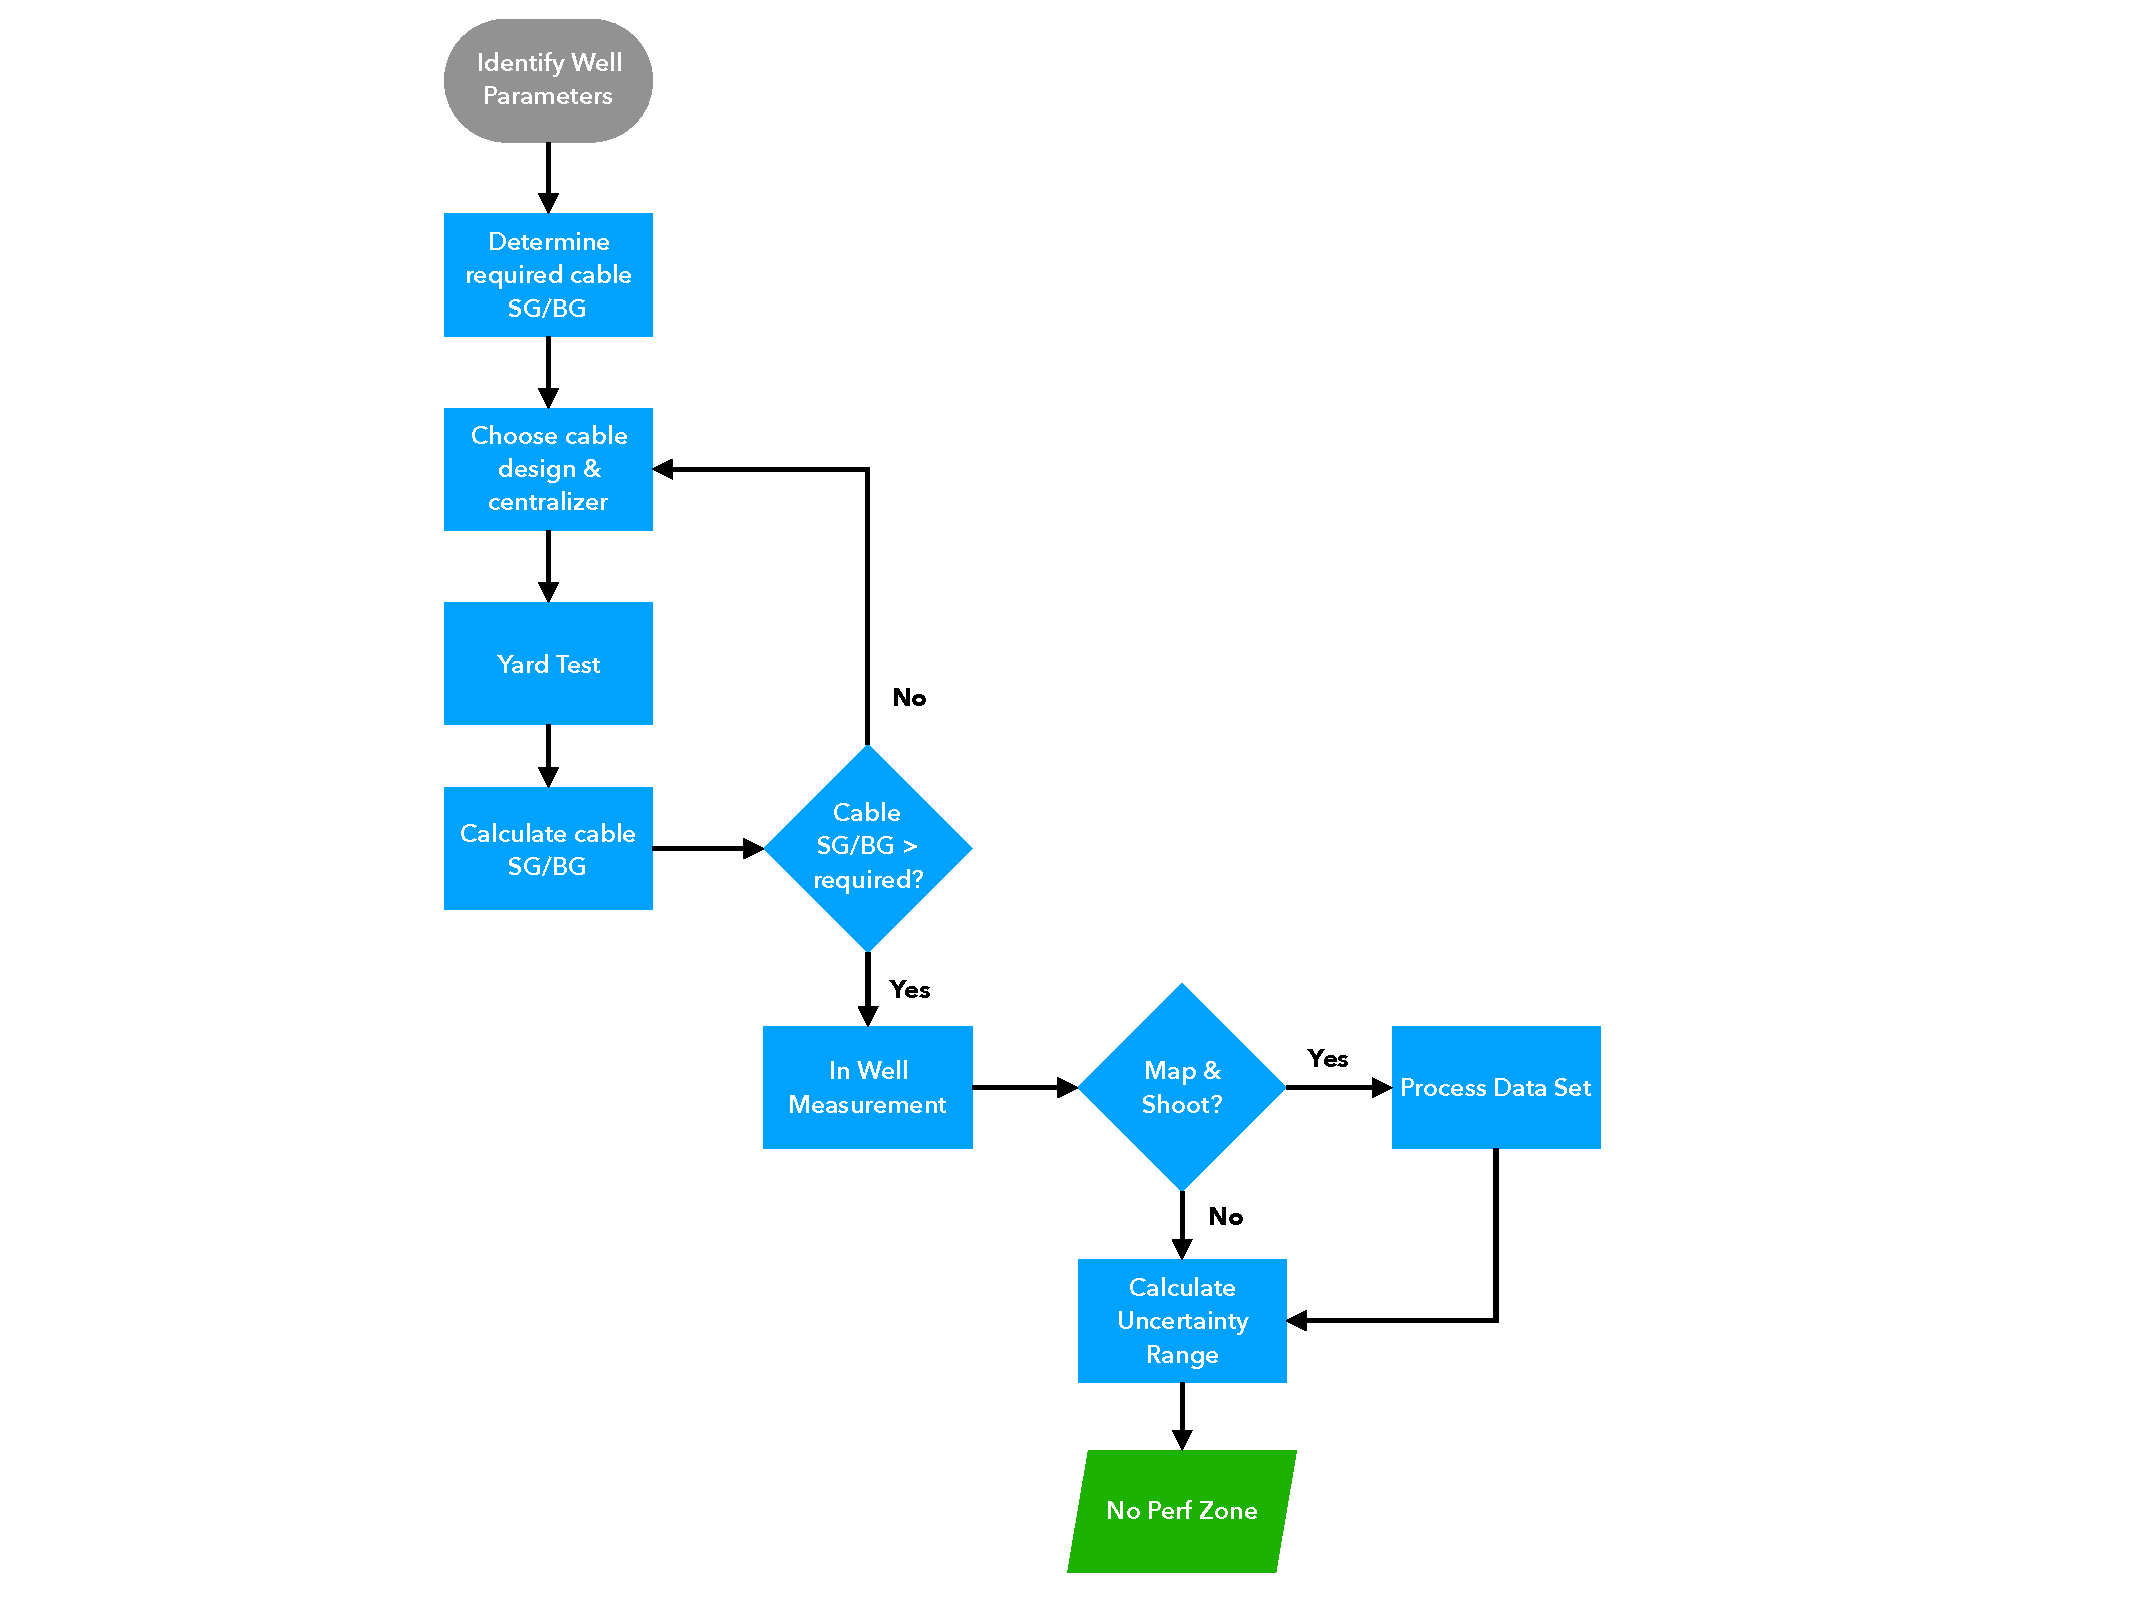
\includegraphics[width=1.0\textwidth]{figures/flow_chart.pdf}
\end{figure}

\begin{figure}[ht!]
    \caption{Schematic of the cable/casing configuration with the identified "no perforation zone" (NPZ).}
    \label{fig:well_schematic}
    \centering
    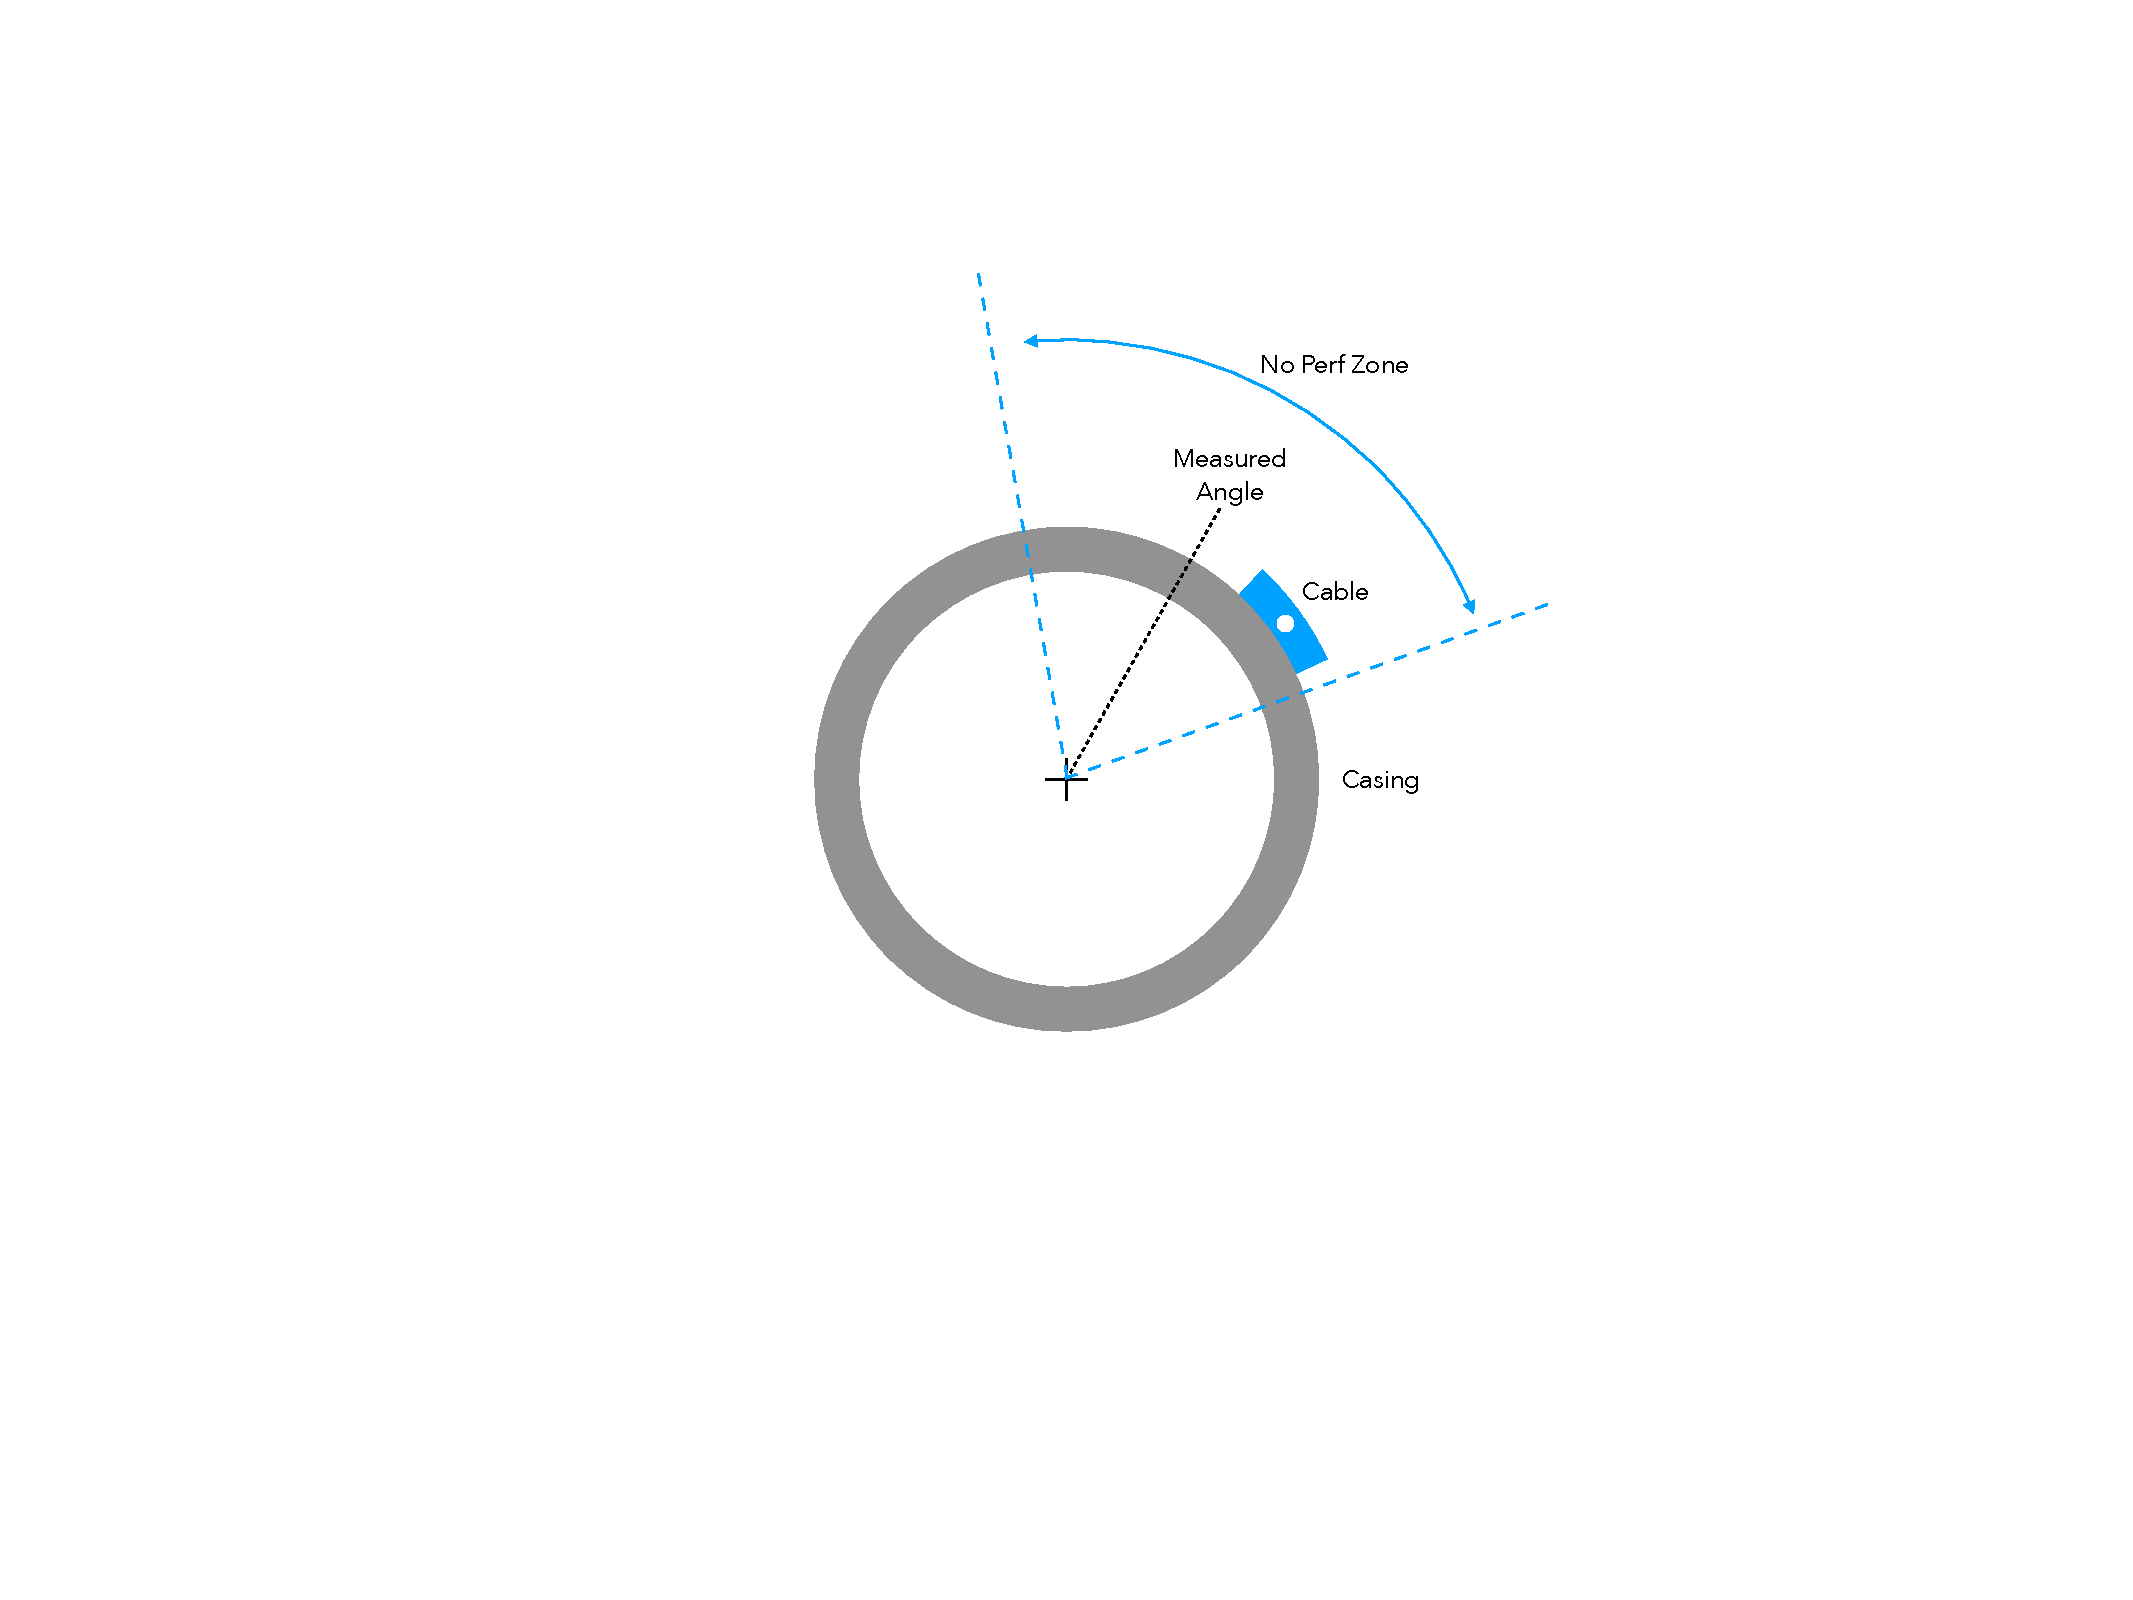
\includegraphics[width=1.0\textwidth]{figures/well_schematic.pdf}
\end{figure}

\section{Step 1: Identify well parameters}
\label{step_1}
The workflow begins by identifying the well parameters and perforation job requirements.  Below is a list of the parameters that influence the NPZ.

\begin{enumerate}
	\item Well orientation - Depending on the method used in the magnetic orientation tool to determine tool orientation, the measured relative bearing is only accurate when the well deviates from vertical.  The motor bearing angle should be used with caution as there is significant angular slip with each rotation. 
	\item Casing material - The signal strength of the tool is influenced by the magnetic properties of the casing.  As a rule of thumb, the measured signal is stronger with carbon steel casing than 13Cr casing.
	\item Casing dimensions - The casing diameter and wall thickness influences the measured signal.  As a rule of thumb, the measured signal is stronger in smaller diameter casing and thinner walls.
	\item Magnetic orientation tool - Though the three main tools (WPP, DC-MOT, and Halliburton) have similar operating principles, the tool operating parameters may be different and will lead to diffent measured signals.
	\item Perforating mode - Is the perforating job point and shoot or map and shoot.  Map and shoot mode can be post-processed to provide a tigher NPZ.
	\item Perforating phasing requirement - Smaller phasing requirements such as 60\textsuperscript{o} phasing require stronger cable signals and lower background signals.  
	\item Available centralizers - Centralization of the tool heavily influences the background signal.  Properly sized centralizers that include rollers help minimize the background signal.  
\end{enumerate}

\section{Step 2: Determine required SG/BG}\label{section:required_sgbg}
The phasing requirements sets a minimum cable signal to background ratio (SG/BG) that must be achieved to ensure high confidence in not damaging the cable.  Based on the phasing requirement specified in section \ref{step_1}, use the graph shown in Fig. \ref{fig:max_error_graph} to identify the target minimum SG/BG needed.  The graph is based on the theoretical model described in Eq. \ref{eq:angle_limits} of the appendix.  An additional safety factor can be applied to account for variations in measurement parameters.  Note that, as shown in Section \ref{section:angle_bounds} of the appendix, if $SG/BG<1$, the maximum angular error is $\pm180\degree$, which means the probability to damage the cable during perforations is completely random.  


\begin{figure}[h!]
    \caption{Graph showing the maximum error in the cable position as a function of the cable signal to background ratio.  The inset zooms in on the error range up to 90\textsuperscript{o}.}
    \label{fig:max_error_graph}
    \centering
    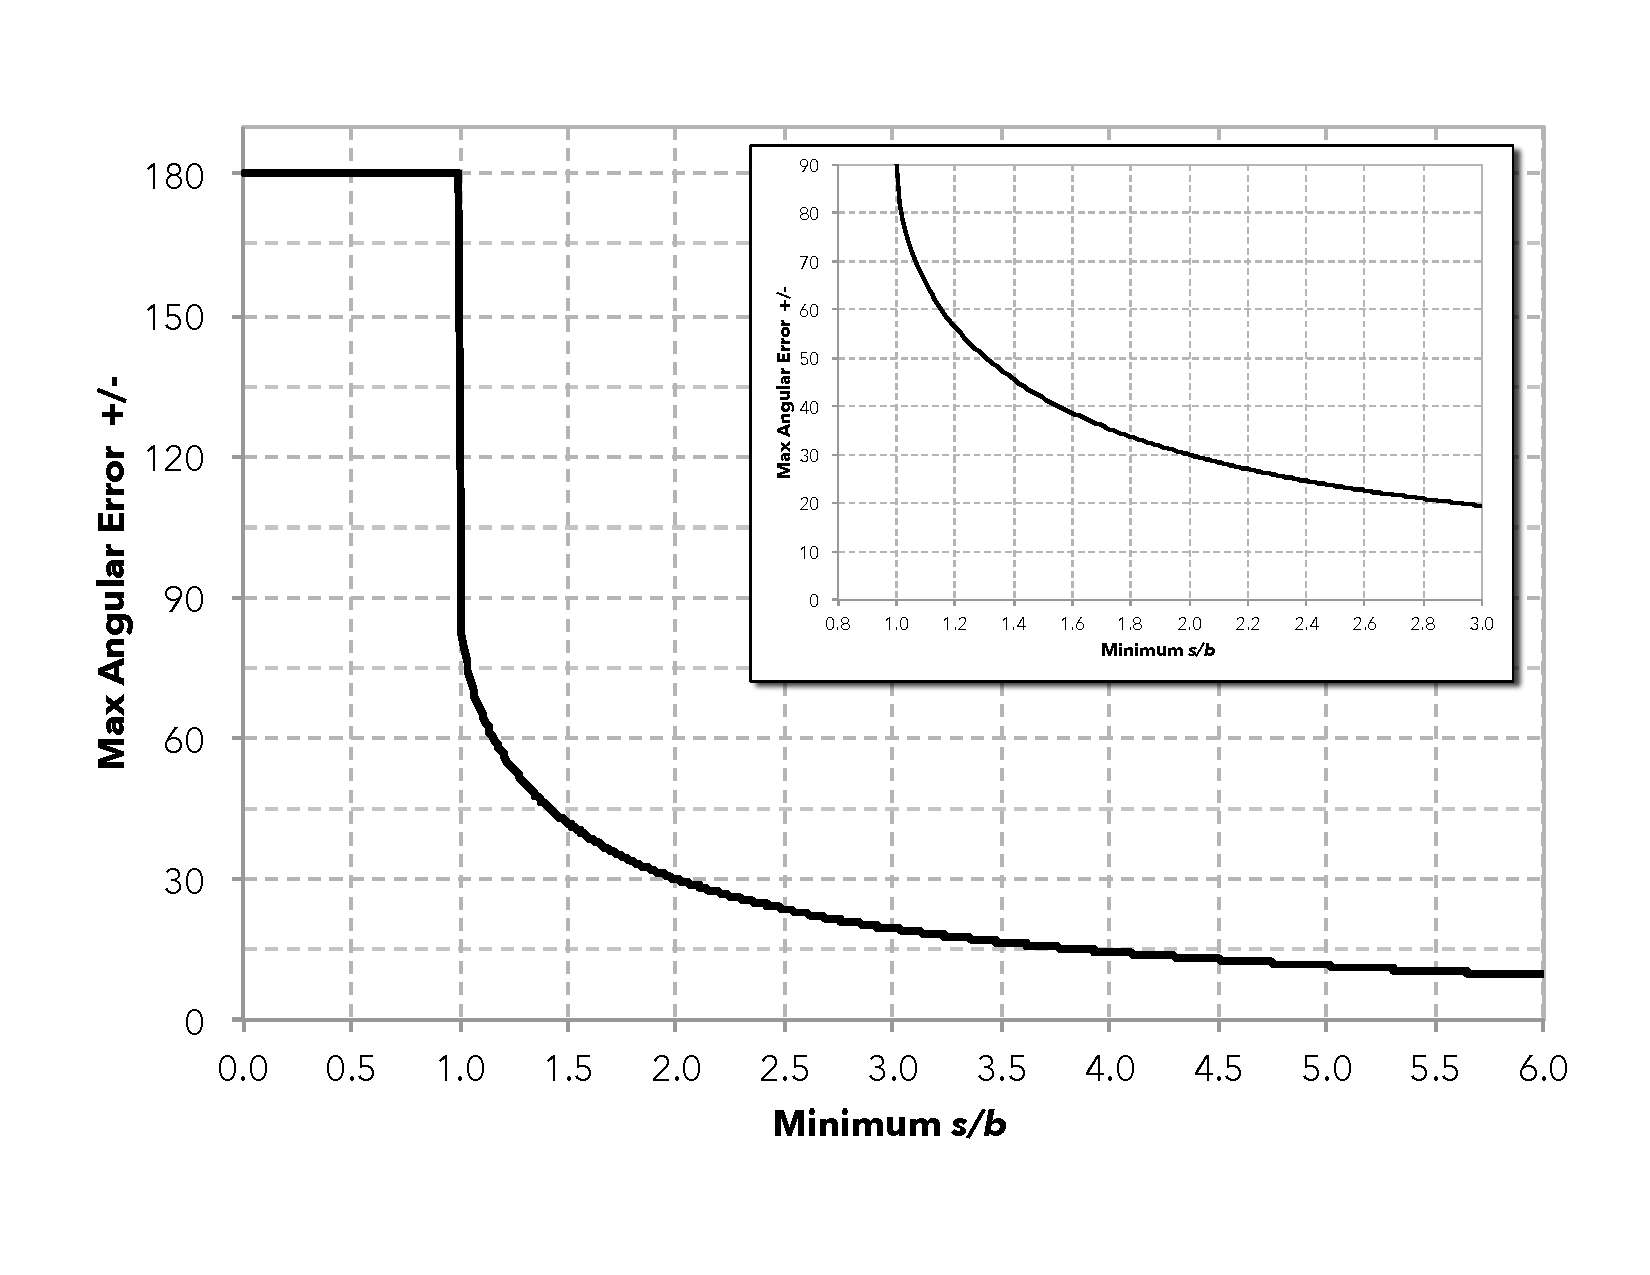
\includegraphics[width=1.0\textwidth]{figures/max_error_vs_sgbg.pdf}
\end{figure}

\paragraph{}
\textbf{Example:} If 60\textsuperscript{o} phasing is required, the maximum allowable angular error is $\pm$ 30\textsuperscript{o}.  Based on the graph, $\pm$ 30\textsuperscript{o} corresponds to an $SG/BG=2$.  Applying a $1.2$ safety factor yields a minimum target $SG/BG = 2.4$.

\section{Step 3: Identify Acculocate Cable Options}
Next, identify 1 to 2 Acculocate cable options.  Fig. \ref{fig:cables} shows examples of Acculocated cable designs.  Below is a list of design factors that increase the measured cable strength.  If available, refer to data from previous measurements of the same cable and similar well parameters to aid the selection. 

\begin{enumerate}
    \item Higher magnetic permeability material - Steel wire rope relies on the magnetic permeability of worked steel which is not very high.  The Acculocate technology deploys grain oriented electrical steel (GOES) strips which has significantly higher magnetic permeability along side structural steel bars (LPC design).  
    \item More layers of GOES strips - Adding additional layers of GOES strips improves signal.  However, mechanical issues arising from coiling multiple strips may arise.  Current Acculocate designs use 1 to 2 layers.
    \item Wider GOES strips - Increasing the width of the GOES strips improves signal but there is a a point of diminishing returns.  Current Acculocate designs use 0.5" to 0.75" wide strips.
\end{enumerate}

\begin{figure}[h!]
    \centering
    \caption{Examples of Acculocate cable designs that incorporate LPC with GOES strips.}
    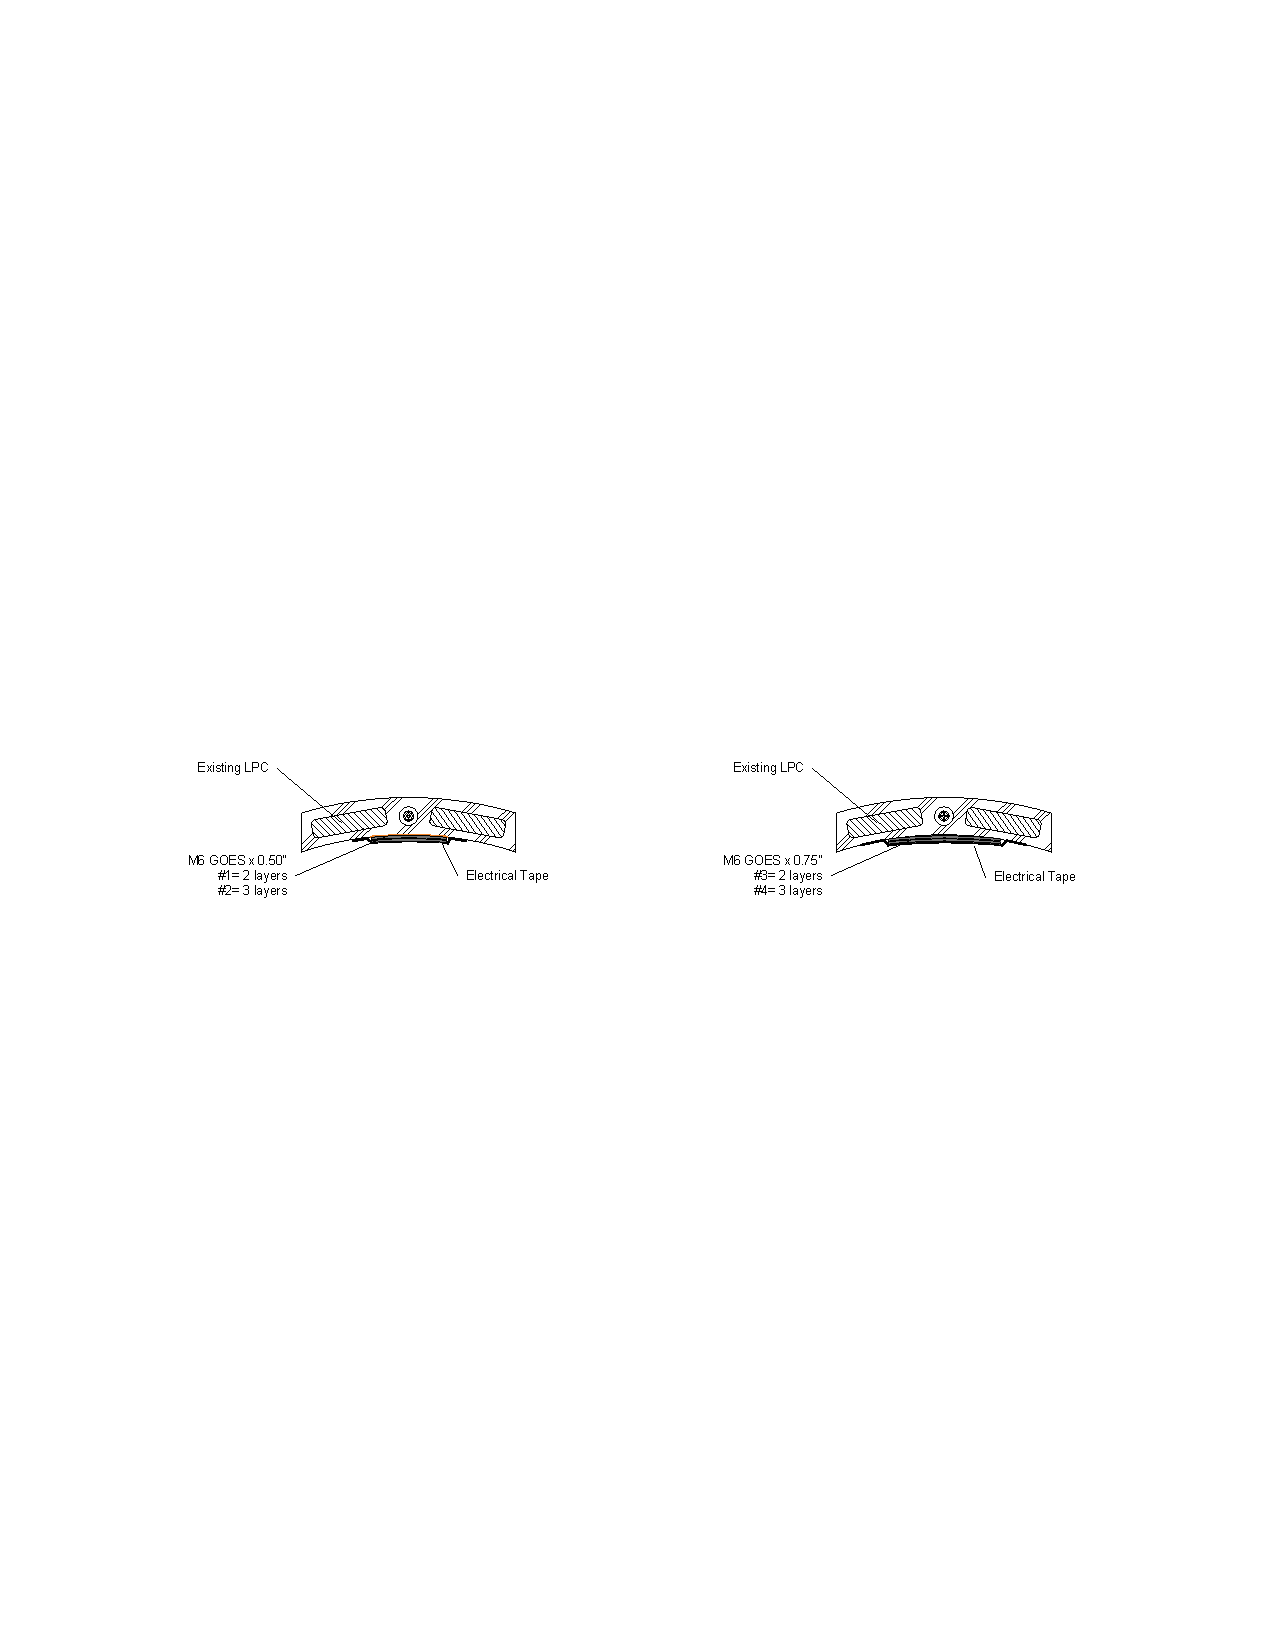
\includegraphics[width=1.0\textwidth]{figures/acculocate_cables.pdf}
    \label{fig:cables}
\end{figure}

\section{Step 4: Conduct Yard Test}

\subsection{Testing overview}
Because there is currently limited data on both cable and background strength across the many parameters that influence the measurement, we recommend conducting a controlled yard test to determine the adequacy of the Acculocate cable to meet the phasing requirements of the perforation job.  Testing should be done prior to the perforation job and replicate the well conditions as close as possible.  Testing generally lasts 1 full day.  The measured span and angle can be recorded in the template spreadsheet.  It's good practice to also obtain PDF and LAS files of the tool output logs.  If possible, create individual LAS files for each test condition.  

\subsection{Equipment needed}
The following equipment is needed for the test.  

\begin{enumerate}
    \item 40 feet of each Acculocate cable option
    \item Magnetic orientation tool and operating crew
    \item 1-2 joints of casing
    \item Selected centralizers
    \item Crane
    \item Pipe stands
    \item Duct tape
    \item Marker
\end{enumerate}

\begin{figure}[h!]
    \centering
    \caption{The measurements steps and corresponding cable positions for the yard test}
    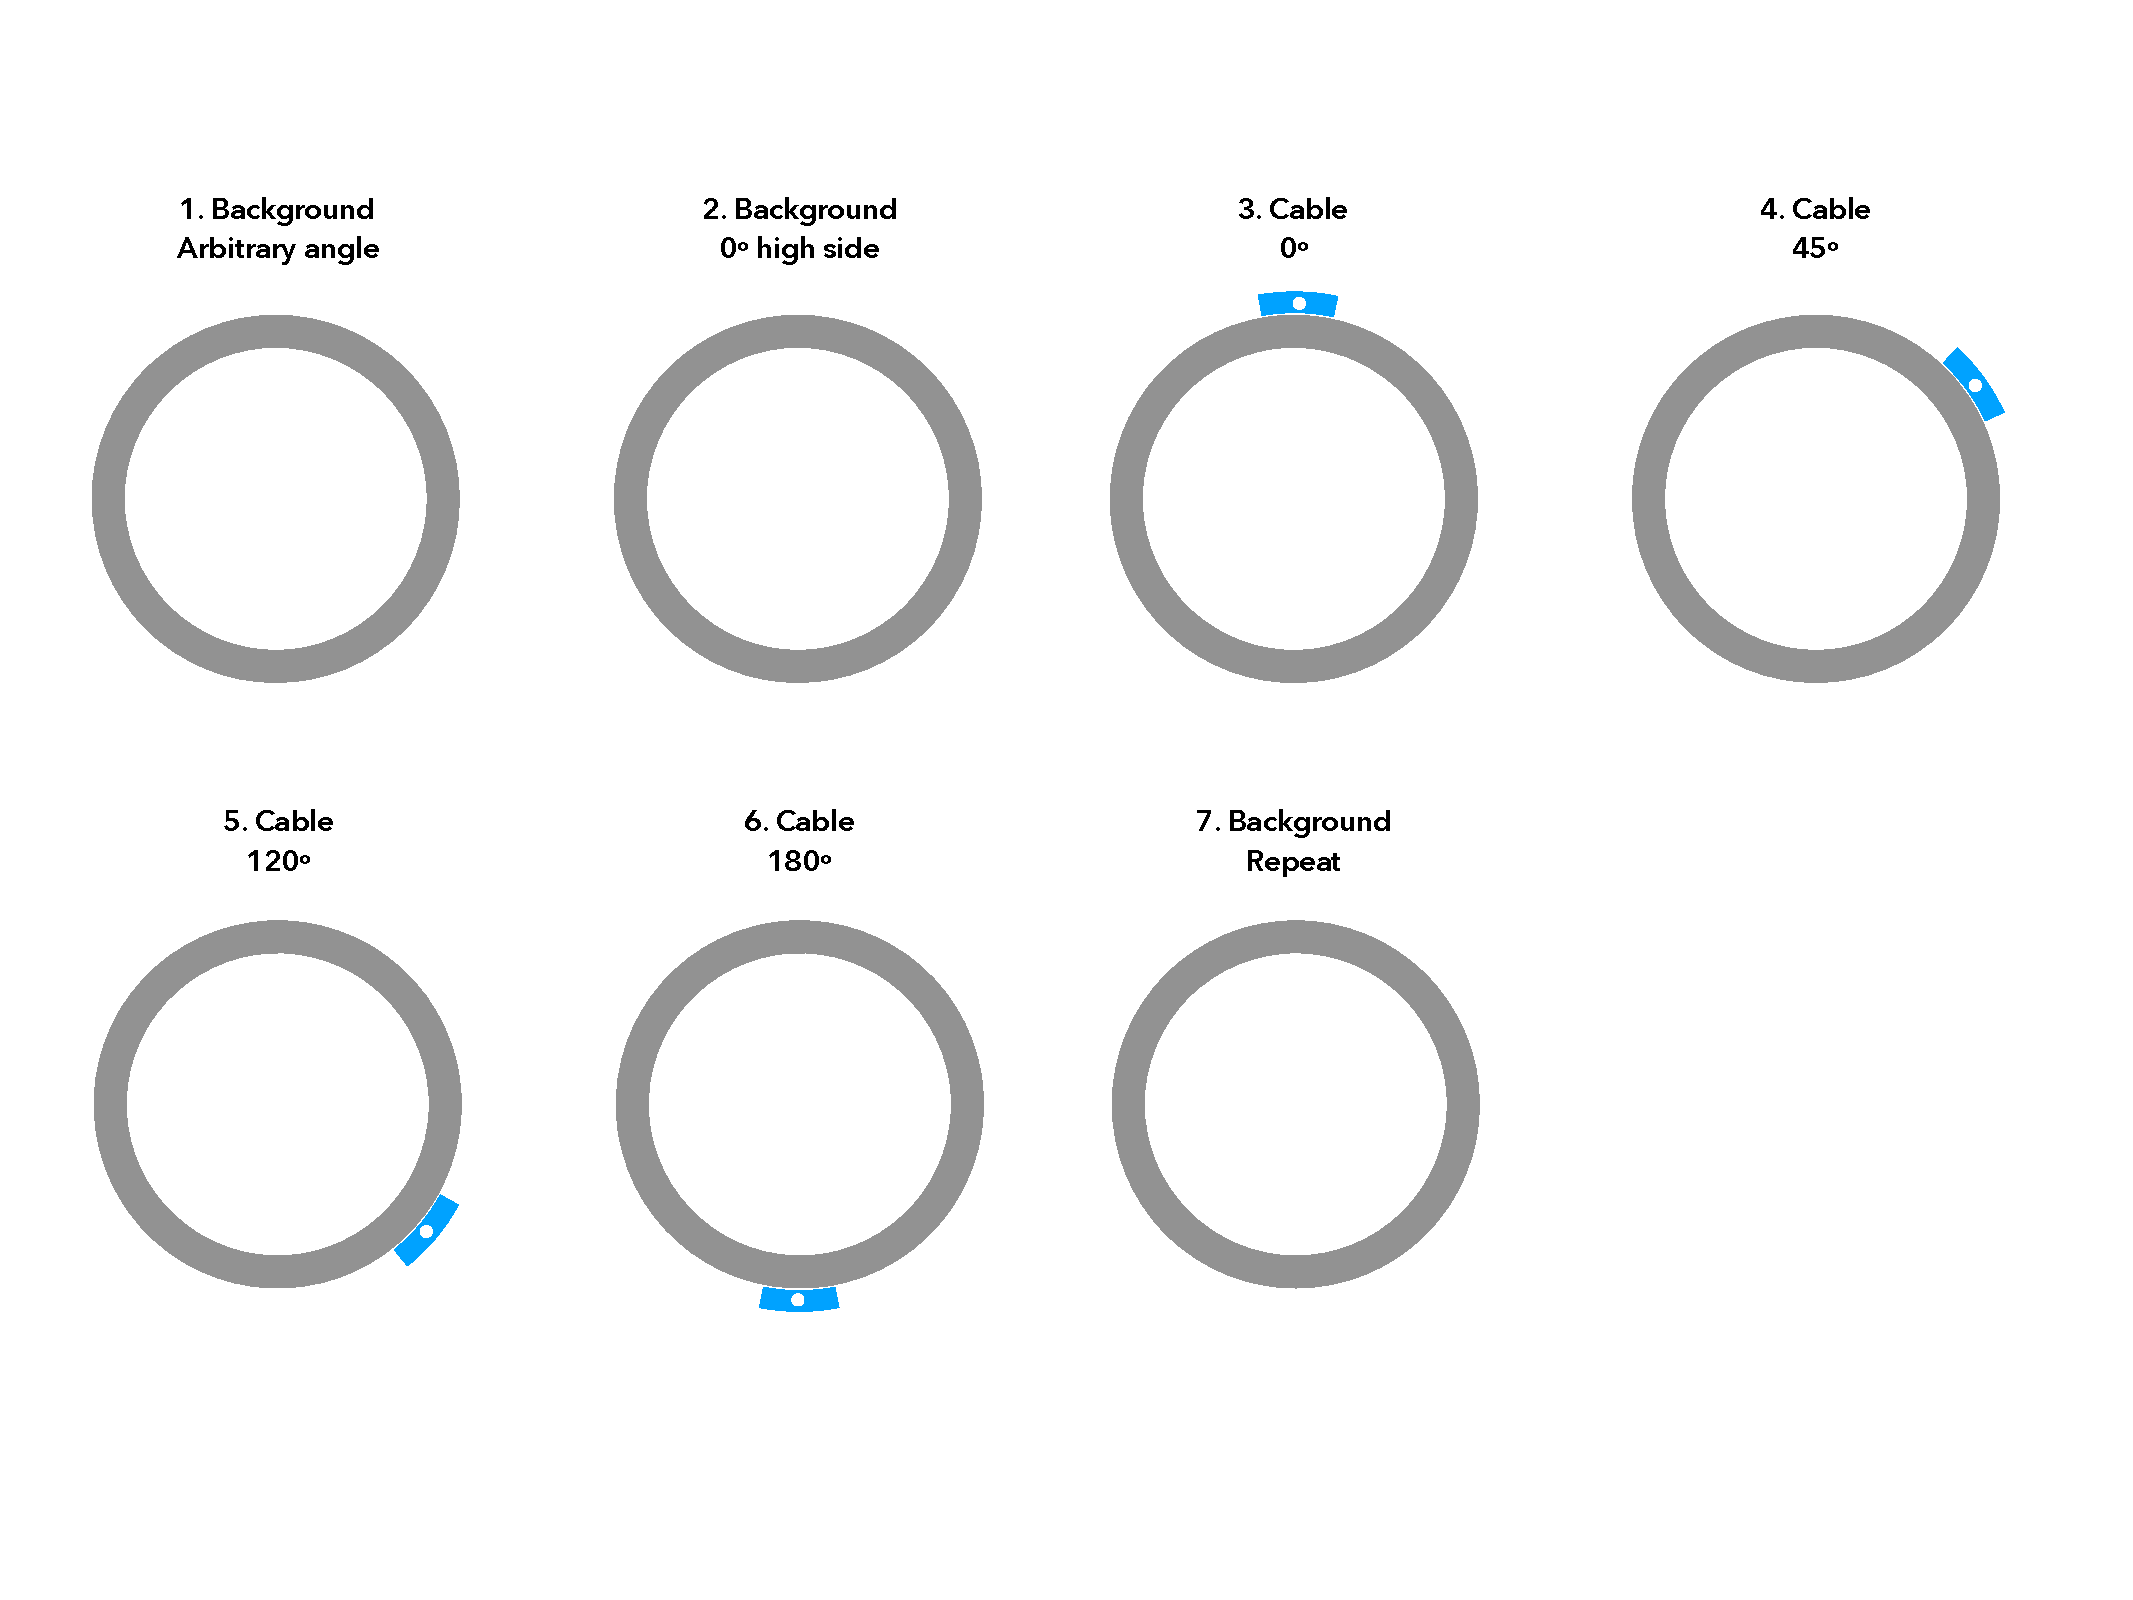
\includegraphics[width=1.0\textwidth]{figures/calibration_steps.pdf}
    \label{fig:calibration_steps}
\end{figure}

\subsection{Testing protocol}
\begin{enumerate}
    \item With both joints on the pipe stands, identify and mark the midpoint along the length of the two joints.
    \item Insert the tool with the centralizers into joint 1 such that the measurement location matches with the marked midpoint.  No cables should be attached to the casing at this point.
    \item Raise the casing to the specified well angle.
    \item Perform measurement and note measured span and angle in template spreadsheet under Test {\#}1 (Fig.\ref{fig:calibration_steps}).  Mark the measured angle on the OD of the casing as 0\textsuperscript{o}.  This is the heavy side.  
    \item Continue to circumfrentially mark the OD of the casing at 45\textsuperscript{o}, 120\textsuperscript{o}, and 180\textsuperscript{o} relative to 0\textsuperscript{o}.
    \item Rotate the casing such that 0\textsuperscript{o} is oriented at the top (heavy side and high side coinciding.)
    \item Repeat measurement and note measured span and angle under Test {\#}2.
    \item Lower casing and attached cable to the casing along its full length  at 0\textsuperscript{o}.  Secure with duct tape.
    \item Raise the casing to the well angle with 0\textsuperscript{o} oriented at the top. Repeat measurement and note measured span and angle under Test {\#}3.
    \item Move and secure cable at 45\textsuperscript{o}.  Repeat measurement and note measured span and angle under Test {\#}4.
    \item Move and secure cable at 120\textsuperscript{o}.  Repeat measurement and note measured span and angle under Test {\#}5.
    \item Move and secure cable at 180\textsuperscript{o}.  Repeat measurement and note measured span and angle under Test {\#}6.
    \item Remove the cable and remeasure the blank casing (background) with 0\textsuperscript{o} oriented at the top.
    \item Repeat cable measurement set with other Acculocate cable options or centralizers.
    \item If time allows, repeat full measurement set on joint \#2.
\end{enumerate}

\section{Step 5: Calculate Cable Signal}\label{section:step_5}
Using these measurements from the yard test, we can calculate the cable and background signal strength along with SG/BG.  The spreadsheet template does the calculation with the entered measurements and estimates upper and lower bounds for SG/BG. 

\paragraph{}
The background signal value is an average of blank casing measurements.  The cable signal strength is calculated for each measurement using
\begin{equation}
    s = m \cos\left(\theta_s-\theta_m\right) - b\cos\left( \theta_s-\theta_b\right)
\end{equation}

where 
\begin{align*}
    s &= \text{cable signal amplitude}\\
    b &= \text{background signal amplitude}\\
    m &= \text{measured signal amplitude}\\
    \theta_s &= \text{cable angle}\\
    \theta_b &= \text{background angle}\\
    \theta_m &= \text{measured angle.}\\
\end{align*}

\paragraph{}
The upper and lower bounds for SG/BG are calculated based on the variation of the signal from the different cable locations.  Because of the limited data set, this is by no means meant to be statistically significant upper and lower bounds.  It is simply an estimate based on the current measurement set.  If a statistically significant amount of data is eventually collected, a proper statistical approach could be implemented.  This is described in Appendix X.

\paragraph{}
The estimated lower bound for SG/BG must now be compared to the target SG/BG from Section \ref{section:required_sgbg}.  If the lower bound for SG/BG is below the target SG/BG, a higher performance Acculocate cable and/or better centralizer should be chosen.  The yard test should be repeated with the new cable and centralizer configuration. 

\paragraph{}
If a selecting a new cable or centralizer is not feasible, there are two alternatives: 
\begin{enumerate}
    \item Relax the phasing requirement.  Use Fig. \ref{fig:max_error_graph} to determine the maximum angular error for the estimated lower bound of SG/BG.  The maximum angular error is also calculated within the template spreadsheet for the estimated SG/BG lower bound.  For example, if the lower bound is 1.2, the maximum error is $\pm$55\textsuperscript{o} which suggests using only 120\textsuperscript{o} phasing to ensure not damaging the cable.
    \item The actual in well NPZ may be less than the maximum angular error.  However this is not known apriori.  Following the in well measurements and calculation of the actual NPZ, final perforating decisions may be made.  
\end{enumerate}

\section{Step 6: In well measurement}
Based on the results of the yard test and calculations, the selected Acculocate cable should be deployed with the casing.  When the perforating jobs are scheduled, the same magnetic orientation tool, measurement parameters, and centralizers from the yard test should also be used.  At each measurement depth, record the measured span and angle.  They can be recorded in the template spreadsheet.  If possible, also acquire the LAS file for each measurement depth.  Note if the measurement depth is near a collar.  They can significantly impact the measurement, increasing the uncertainty of the cable location.  

\section{Step 7: Calculate no perforation zone}
With the measured span and angle, the NPZ can be calculated using Eq.\ref{eq:theta_solution}.  This calculation is provided within the template spreadsheet.  This will be $\pm$ of the measured angle, and its range may be less than the maximum angular error calculated in Step 5.  The perforations should then be directed away from the calculated NPZ. 

\paragraph{}
\textbf{Example:} Given a measured cable and background signal from the yard test of ${2183\pm614}$ and ${900\pm82}$, respectively, and an in well measured span and angle of 2000 and 45\textsuperscript{o}, respectively, the estimated NPZ is 16-74\textsuperscript{o}.  The perforations should be oriented away from this 16-74\textsuperscript{o} angular range.

\paragraph{}
For point and shoot jobs, this calculation can be part of the jobsite workflow and immediately guide the perforation orientation.  For map and shoot jobs, post-job processing can further reduce the range of the NPZ.  This relies on correlating measurements from multiple depths to reduce noise in the measurement.  The map and shoot post-processing can be performed as follows (Fig.\ref{fig:map_shoot}):
\begin{enumerate}
    \item Plot measured span and angle as a function of depth (log orientation).
    \item Remove outliers, many of which will be near the collars
    \item Fit the remaining data points for span and angle to a linear function vs depth
    \item Calculate the $\pm$ NPZ bearing correction based off the beginning and end of the linear fits.
    \item Apply the $\pm$ NPZ bearing correction to the linear fit to create an NPZ band as a function of depth.
\end{enumerate}

\begin{figure}[h!]
    \caption{Plot representing the steps to post-process map and shoot data to generate NPZ bands as a function of depth.}
    \centering
    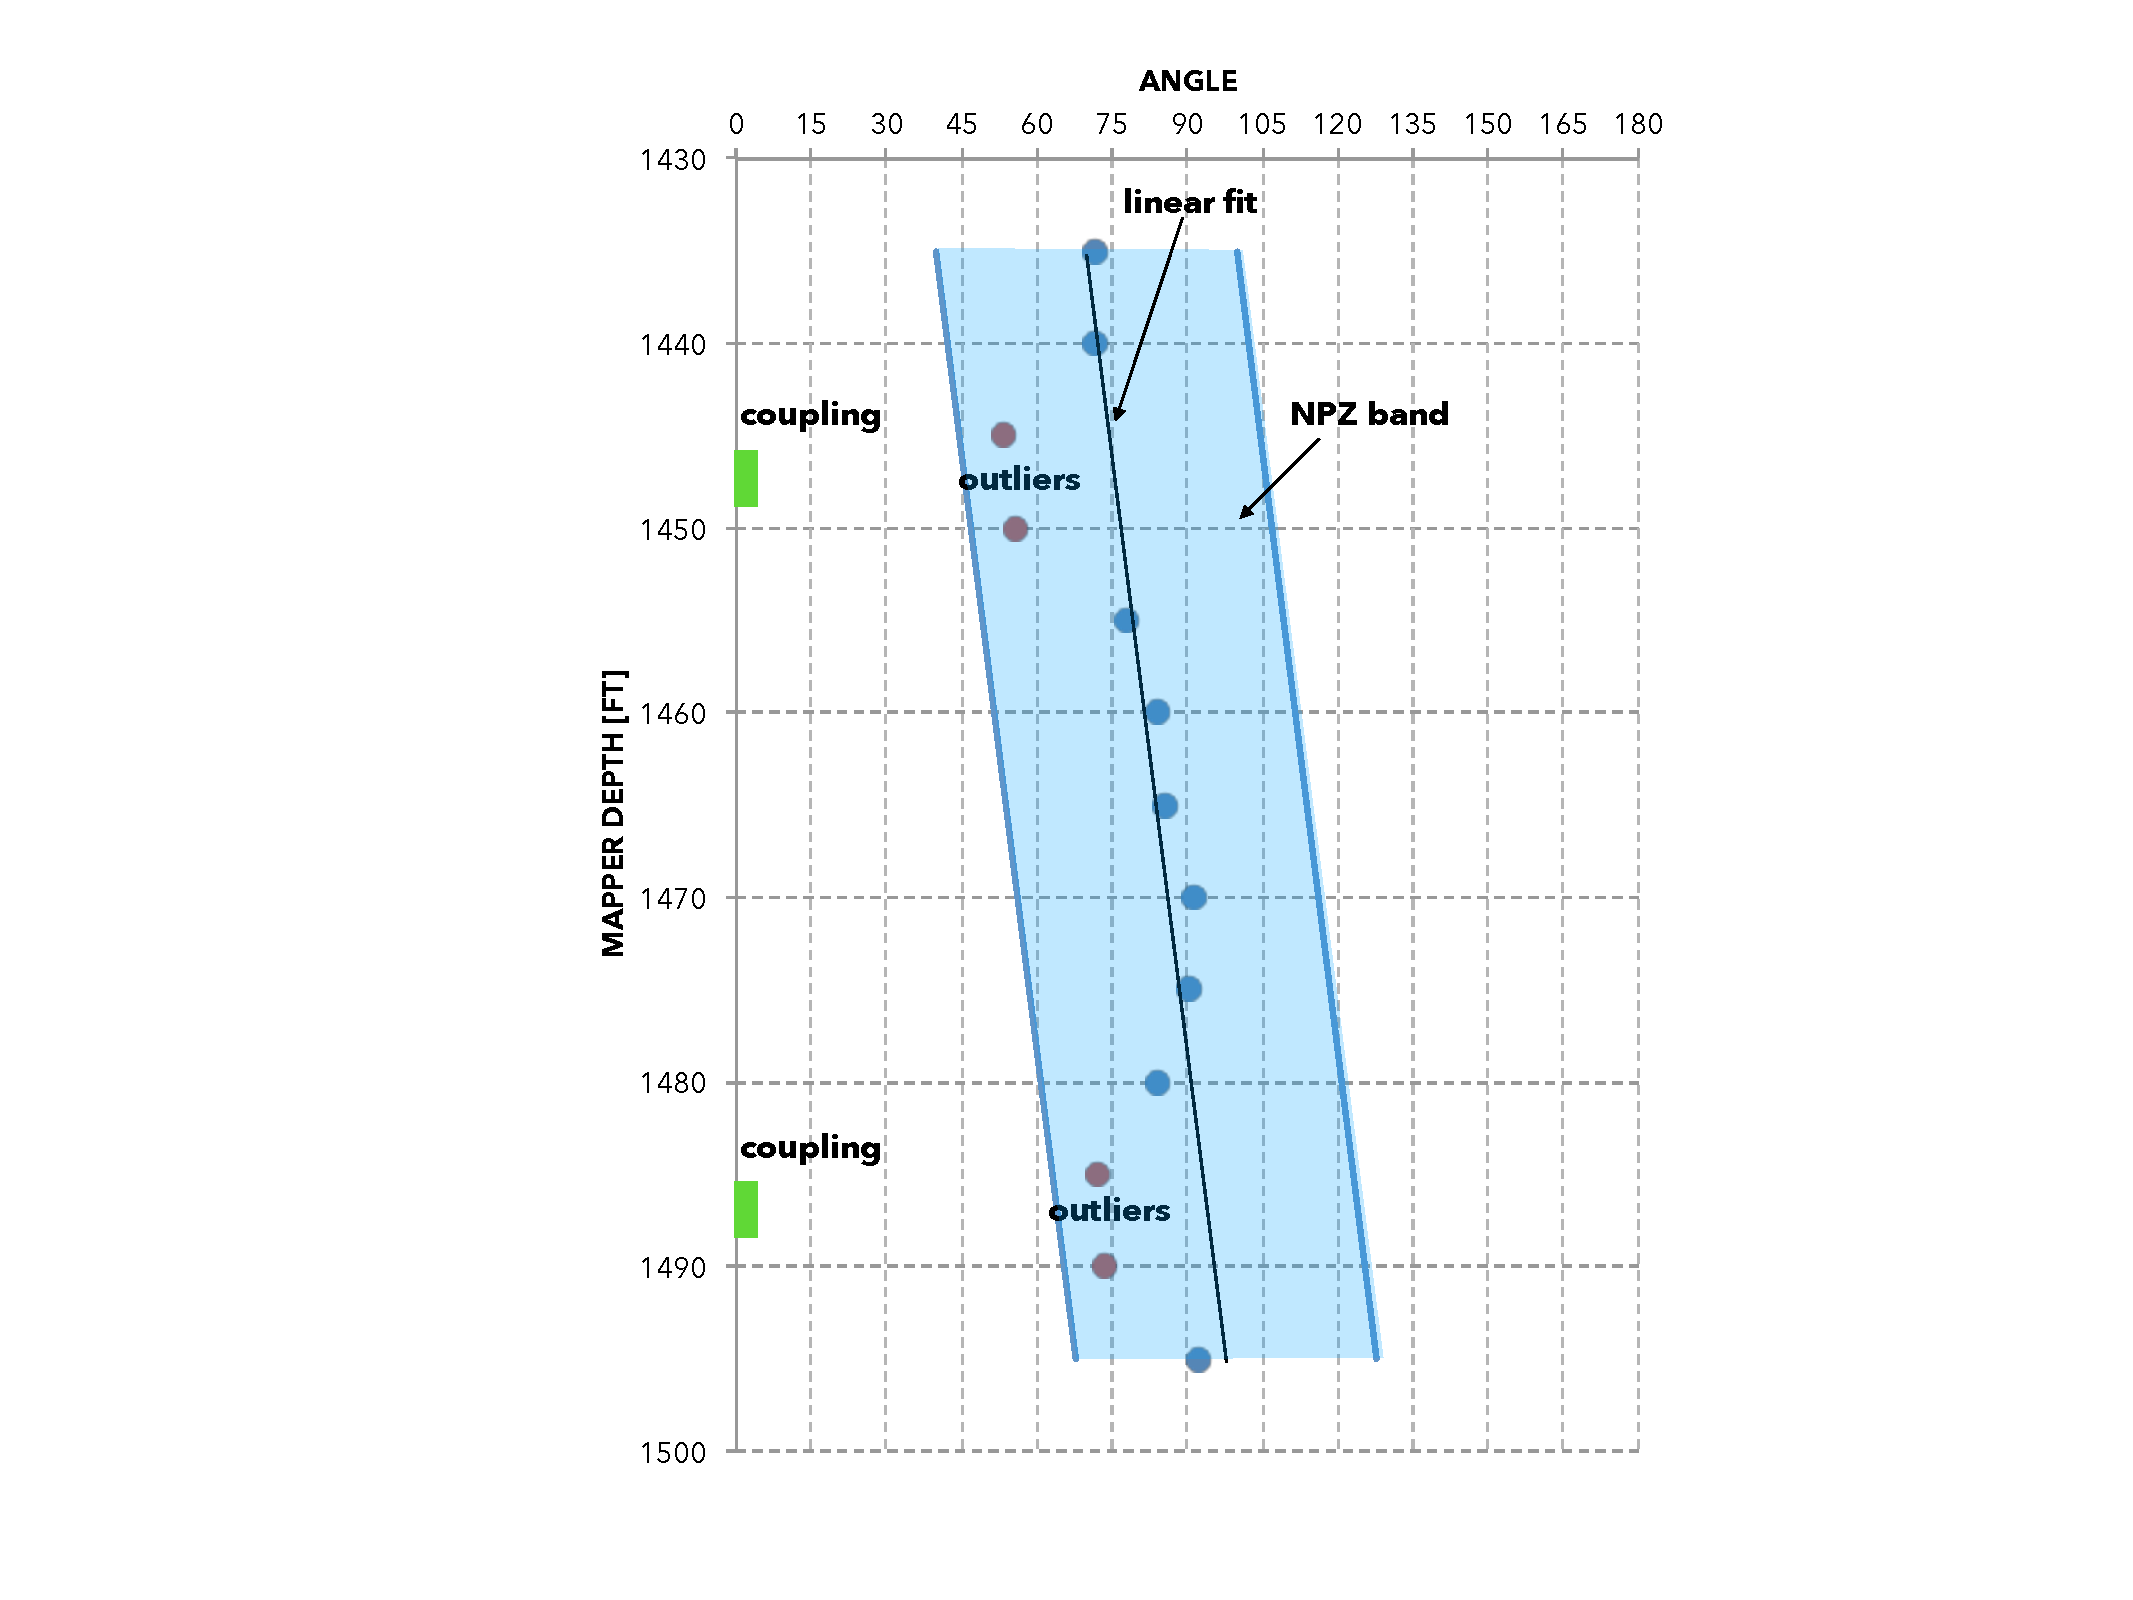
\includegraphics[width=1.0\textwidth]{figures/map_shoot.pdf}
    \label{fig:map_shoot}
\end{figure}












\begin{appendices}

\section{Estimating the Bearing Correction}
\subsection{The Bearing Correction}
The signal measured within the pipe will vary as a function of angle.  We can break down the source of this signal into two components.  The first component we will call the ``cable signal.''  This is the signal variation caused by the presence of the cable attached to the outside of the pipe.  The second component we will call the ``background signal,'' which arises from all other sources of angular asymmetry in the system.  This is thought to be dominated by imperfect centering of the instrument within the pipe.

\par We model both the background and the cable signals as if they are sinusoidal functions. The total measured signal is then given by

\begin{equation} \label{eq:trig_sig}
    s = C \sin\left(\theta + \phi_c\right) + B \sin\left(\theta + \phi_b\right),
\end{equation}
where
\begin{align*}
        S &= \text{total signal amplitude} \\
        C &= \text{cable signal amplitude} \\
        B &= \text{background signal amplitude.} \\
        \phi_c &= \text{the phase of the cable signal}\\
        \phi_b &= \text{the phase of the background signal}\\
\end{align*}


\begin{figure}[H]
  \caption{An example model.  In this example, we arbitrarily choose amplitudes and phases for the cable and background components such that  $s = \sin\theta + 0.25 \sin\left(\theta -135\degree\right)$
  }
  \label{fig:sigs_vs_bearing}
  \centering
  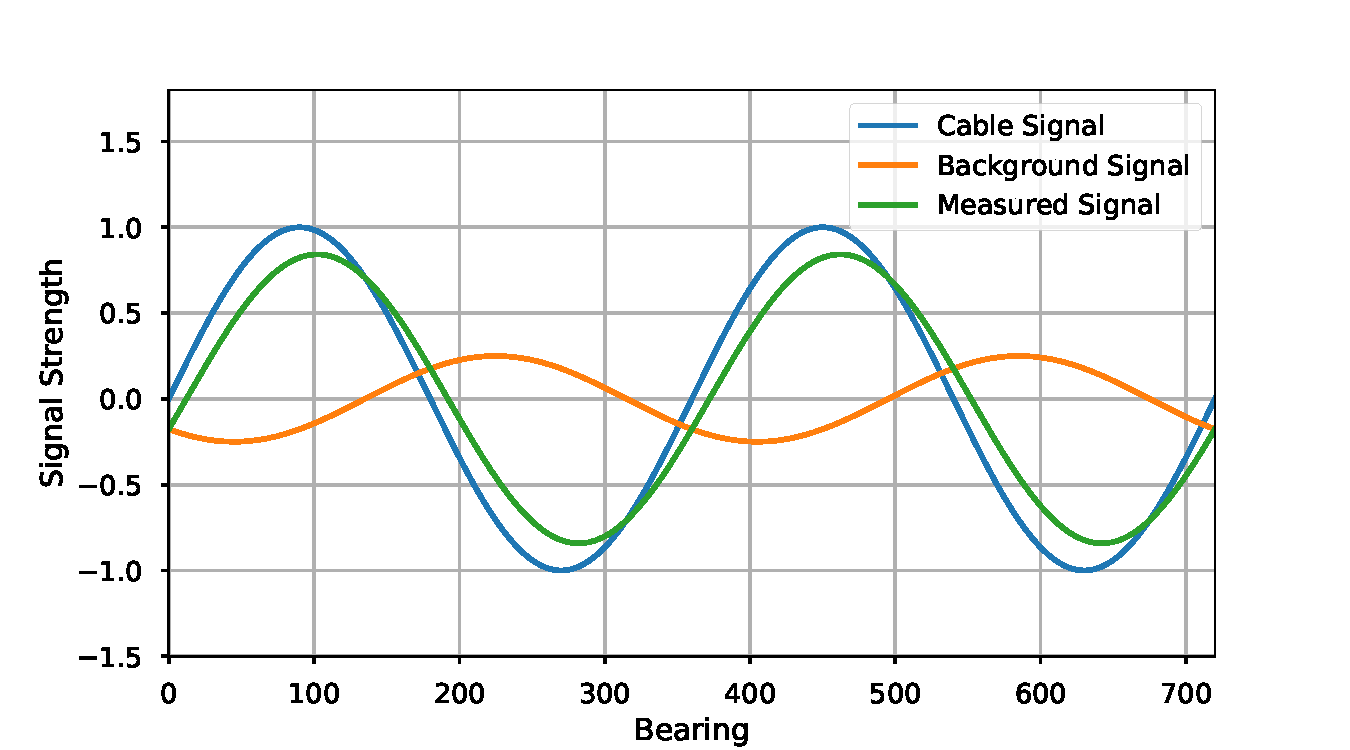
\includegraphics[width=1.0\textwidth]{figures/sigs_vs_bearing.pdf}
\end{figure}

We arbitrarily construct an example model where we set $C=1$, $B=.25$, $\phi_c=1$, and $\phi_b=135\degree$. Figure \ref{fig:sigs_vs_bearing} shows this model plotted as a function of bearing angle.

Although a plot of amplitude vs angle is useful, a better way of visualizing the problem is to transform it to a phasor representation.  To do this, recall that
\begin{align}
        \cos{\theta} &= Re\left(e^{i\theta}\right) \\
        \sin{\theta} &= Im\left(e^{i\theta}\right). \\
\end{align}
This lets us visualize the components of the measured signal as if they were two-dimensional vectors in the complex plane, (i.e. phasors). Fig. \ref{fig:phasor_base} shows our example problem visualized with phasors.

\begin{figure}[h]
  \caption{
  The phasor representation of the example model from Figure \ref{fig:sigs_vs_bearing}. $s$ is the cable-signal phasor, $b$ the background phasor and $m$ the measured phasor.  The bearing-correction angle, $\theta$, is the angle between the measured and cable signals.  Note that we can only determine the magnitude of the angle, but not the sign.  The phasor relationships shown in solid lines are indistinguishable from those shown by the dashed lines.  This model provides no information for distinguishing between the $\pm\theta$ solutions}
  \label{fig:phasor_base}
  \centering
  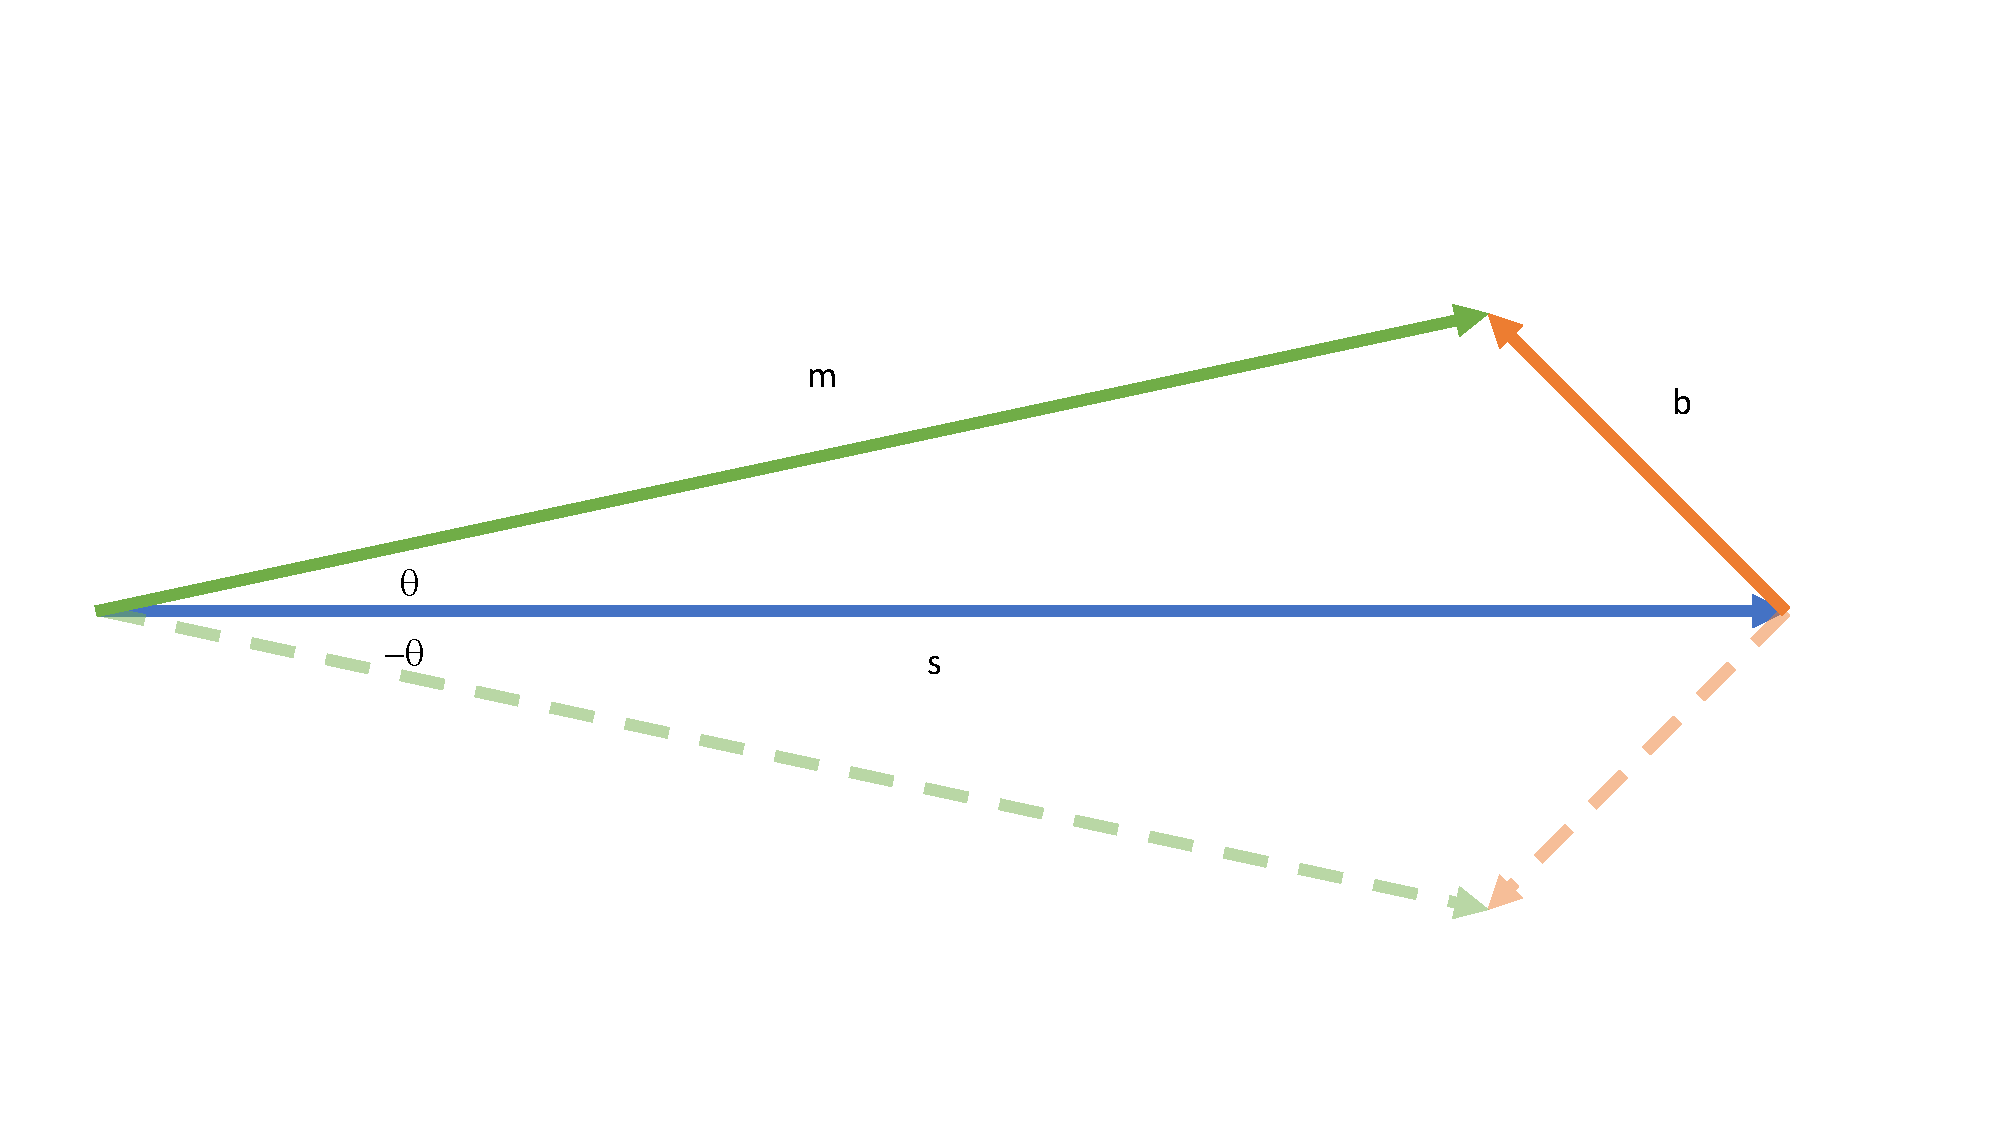
\includegraphics[width=1.0\textwidth]{figures/phasor_base.pdf}
\end{figure}
Our objective is to find the bearing correction that must be applied to the measured signal in order to arrive at the true cable signal. In this representation, the correction angle, $\theta$, is readily obtained from the law of cosines.
\begin{equation} \label{eq:law_of_cos}
    \cos\left(\theta\right) = \frac{m^2 + s^2 - b^2}{2ms}
\end{equation}
But since $\cos\left(\cdot\right)$ is an even function of its argument, we are unable to distinguish between solutions having positive and negative $\theta$.  So our solution becomes

\begin{equation} \label{eq:theta_solution}
\theta = \pm \cos^{-1}\left(\frac{m^2 + s^2 - b^2}{2ms}\right)
\end{equation}
where
\begin{align*}
        \theta &= \text{the angle between the measured and cable signals}\\
        s &= \text{cable signal amplitude.}\\
        b &= \text{background signal amplitude} \\
        m &= \text{measured signal amplitude} \\
\end{align*}


\subsection{Placing Bounds on the Bearing Correction Angle}\label{section:angle_bounds}
In this section we will show that the ratio of cable-signal to background-signal ($s/b$) is the most important figure of merit for putting limits on the bearing-correction angle. The larger this ratio, the tighter the limits. We will further prove that there is no limit on the bearing-correction angle when $s/b < 1$.




Figure \ref{fig:angle_limits} shows phasor diagrams for two different configurations superimposed on each other.  The phasors drawn with solid lines represent a configuration where $s>b$.  The measurement is the phasor sum, $m=s+b$.  Since $\alpha$, the angle between $s$ and $b$, can take on any value, the tip of the measurement phasor,  $m$, can lie anywhere on the the solid circle.  In this configuration, the bearing correction angle, $\theta$, is maximized when the measurement phasor, $m$, is tangent to the circle.  By inspecting the diagram and applying trigonometry, we arrive at an expression that limits the bearing-correction angle: 
\begin{equation} \label{eq:angle_limits}
    \left| \theta \right| \leq \sin^{-1}\left(\frac{b}{s}\right).
\end{equation}

The phasors drawn with dashed lines represent a configuration for $b > s$.  In this case, the tip of the measurement vector can lie anywhere on the larger dashed circle.  As can be seen, this allows the bearing-correction angle, $\theta$, to take on any value between $0\degree$ and $360\degree$.

\begin{figure}[H]
  \caption{The phasor sums for two different conditions are shown here, one with solid lines, and the other with dashed lines.  In each case, the measured signal ($m$) is the phasor sum of the cable ($s$) and the background ($b$) signals. The angle between the cable and background signals ($\alpha$) can range between $0\degree$ and $360\degree$.  The solid circle represents the locus of all points reachable for fixed $b$ and $s$ when $b < s$.  $\theta$ is maximized when the measurement vector ($m$) is tangent to the circle.  The dashed circle shows the case for $b > s$.  Under these circumstances, $\theta$ can range from  $0\degree$ to $360\degree$. 
  }
  \label{fig:angle_limits}
  \centering
  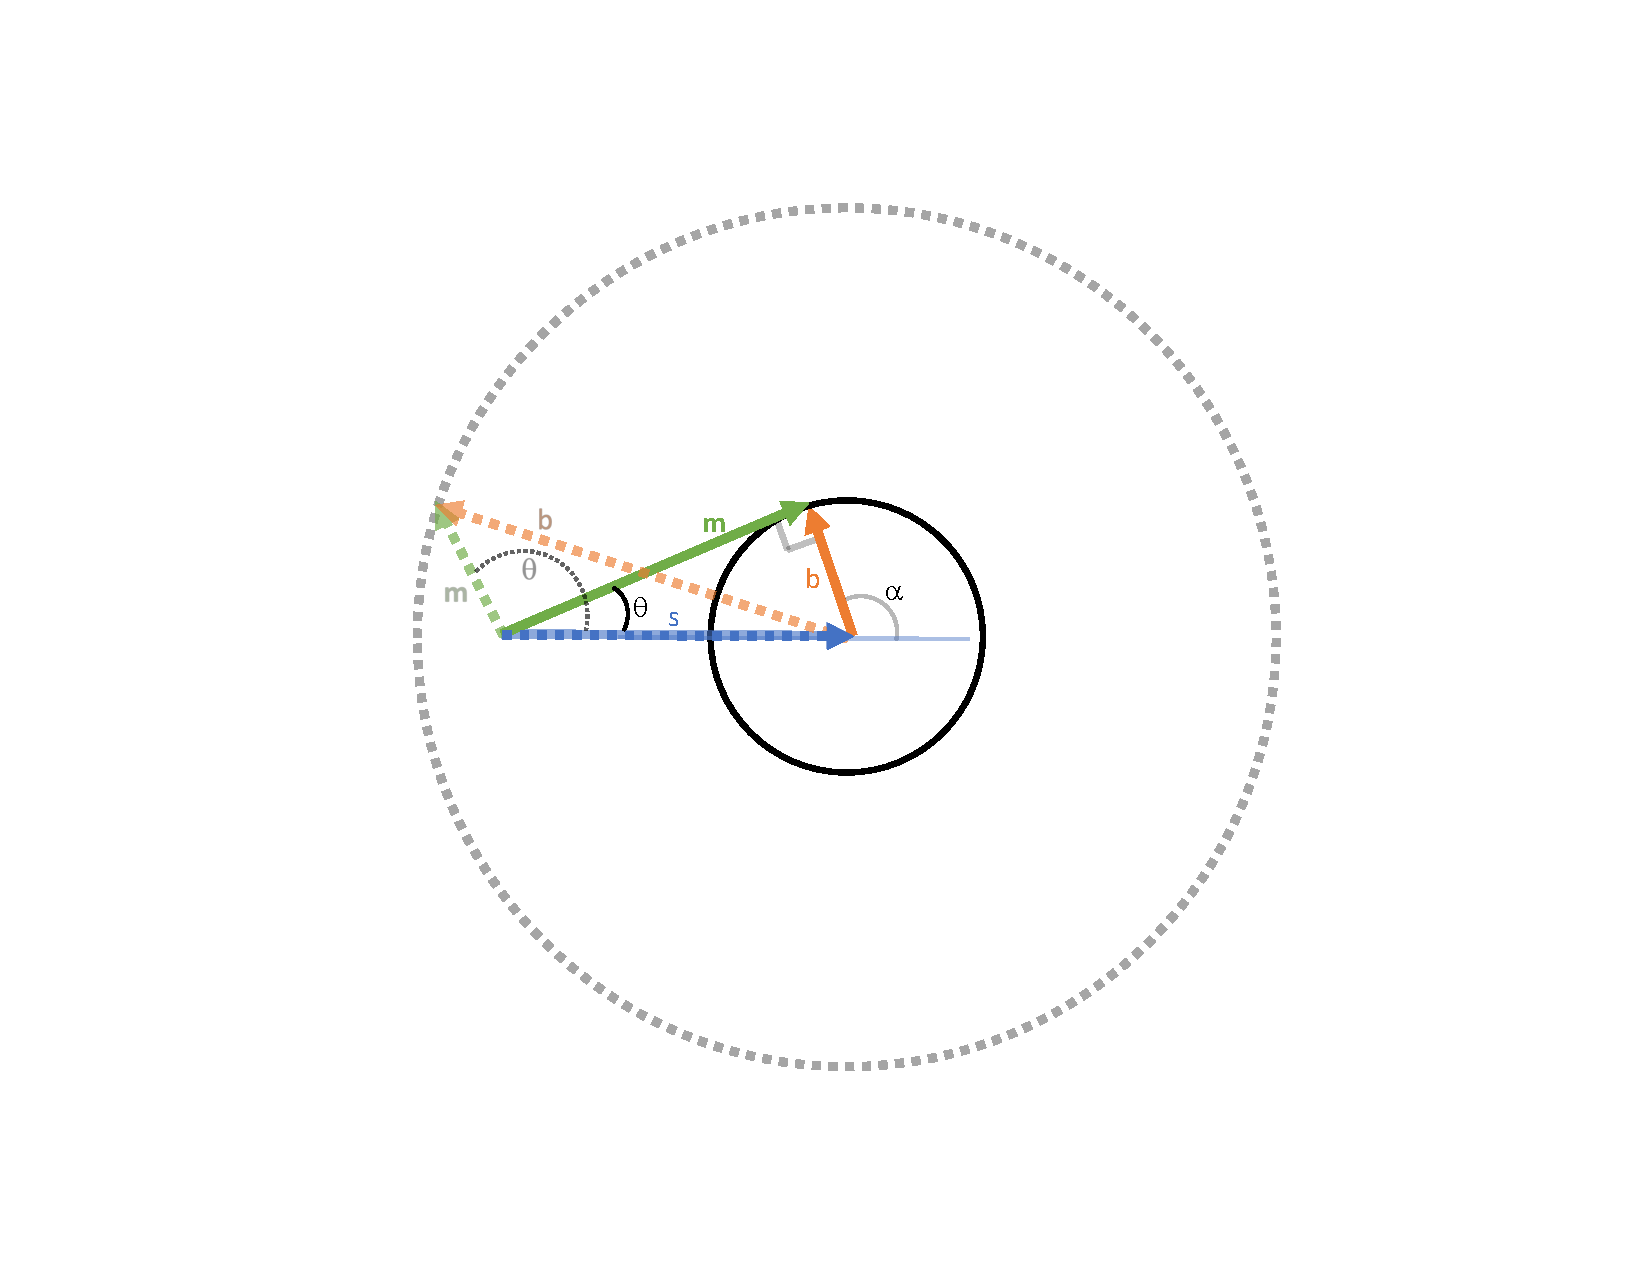
\includegraphics[width=1.0\textwidth]{figures/angle_limits.pdf}
\end{figure}


    
\section{Statistical Constraints on the Bearing Correction Angle}
So far in this appendix we have been able to place limits on the bearing correction angle provided that we are able to reliably quantify the ratio between the cable and background signals.  In practice, this ratio is difficult to nail down exactly. The magnetic properties measured by the Acculocator can change as it is moved along the pipe.  This non-uniformity can cause both the cable and background signals to vary as the position of the instrument changes, and there is no way to determine an exact value for the signal-to-background ratio.  Under these circumstances, the best we can do is describe the cable and background signals with statistical distributions that model real-world variations.

There are any number of statistical distributions we could use to model these variations, but here we select the Gamma distribution.  Like the amplitudes we are modeling, the Gamma distribution is only defined for positive values and can be uniquely specified with a mean and standard-deviation.  Any other distribution meeting these requirements could be used, but we believe the Gamma distribution is a reasonable choice.

Having chosen to model the cable and background signals as Gamma distributions, we will use Monte-Carlo simulation (see Algorithm \ref{monte_algo}) to randomly draw values from our model distributions and propagate those draws through the algebra required to compute the corresponding bearing-correction
\footnote{
    A detail in Algorithm \ref{monte_algo} is not readily apparent and deserves a short explanation.  Given a measurement $m$, it is important to ensure that the random values we draw for $s$, and $b$ are able to form a valid triangle. We use the law of cosines, equation \ref{eq:law_of_cos},  and the fact that $\left|\cos\theta\right| <=1$ to derive the following constraint:
    \begin{equation} \label{eq:bounds}
          \left(m-s\right)^2 \leq b ^ 2 \leq \left(m + s\right)^2.  
    \end{equation}
    
}.
In this way, we can build a statistical distribution capable of placing probabilistic constraints on the bearing-correction angle.
Fig. \ref{fig:correction_hist} shows a histogram of samples generated using Algorithm \ref{monte_algo}.

The histogram of Figure \ref{fig:correction_hist} is useful from a qualitative perspective. The twin peaks, for example, starkly illustrate the model's inability to distinguish between positive and negative correction angles.  However, a plot of the empirical cumulative distribution function (ECDF) provides a far more useful visualization from which confidence bounds can be directly read. Figure \ref{fig:correction_ecdf} shows the ECDF corresponding to the histogram of Figure \ref{fig:correction_hist}.  The shaded regions correspond to the 1-$\sigma$ and 2-$\sigma$ confidence bounds containing $66\%$ and $95\%$ of the probability, respectively.


\begin{figure}[H]
  \caption{
  A histogram of $10^5$ samples generated using algorithm \ref{monte_algo}.  For this simulation, we specified the cable-signal distribution with a mean and standard-deviation of $\mu_s=1900$, $\sigma_s=200$, and the background-signal distribution with a mean and standard-deviation of $\mu_b=900$, $\sigma_b=200$.  In this case the nominal signal-to-background ratio was $2.1$.  The double-hump in the histogram is driven by our inability to distinguish between the positive and negative sign in equation \ref{eq:theta_solution}. Notice how the nominal lower bound on the signal-to-background is $1700/1100 \approx 1.5$.  Using Figure \ref{fig:max_error_graph}, we estimate the bearing-correction bounds to be $\approx40\degree$, which is consistent with the range shown in this histogram. 
  }

  
  \label{fig:correction_hist}
  \centering
  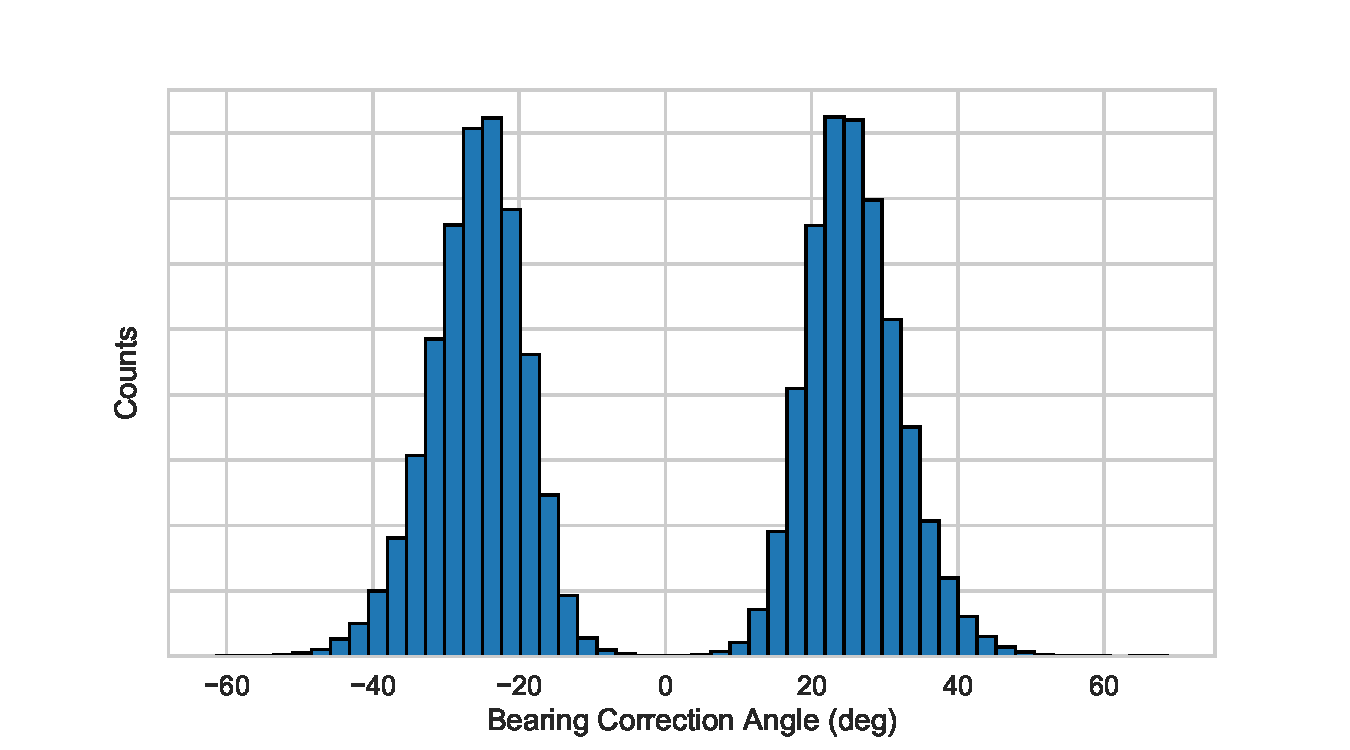
\includegraphics[width=1.0\textwidth]{figures/correction_hist.pdf}
\end{figure}


\begin{figure}[H]
  \caption{
  The empirical distribution function (ECDF) for the same samples shown in Figure \ref{fig:correction_hist}.  ECDF plots are useful for identifying confidence intervals.  For this example, the statistical model provides  $95\%$ confidence that the bearing correction angle will fall within $\pm 37\degree$, and  $66\%$ confidence that it will fall within $\pm 28\degree$.
  }
  \label{fig:correction_ecdf}
  \centering
  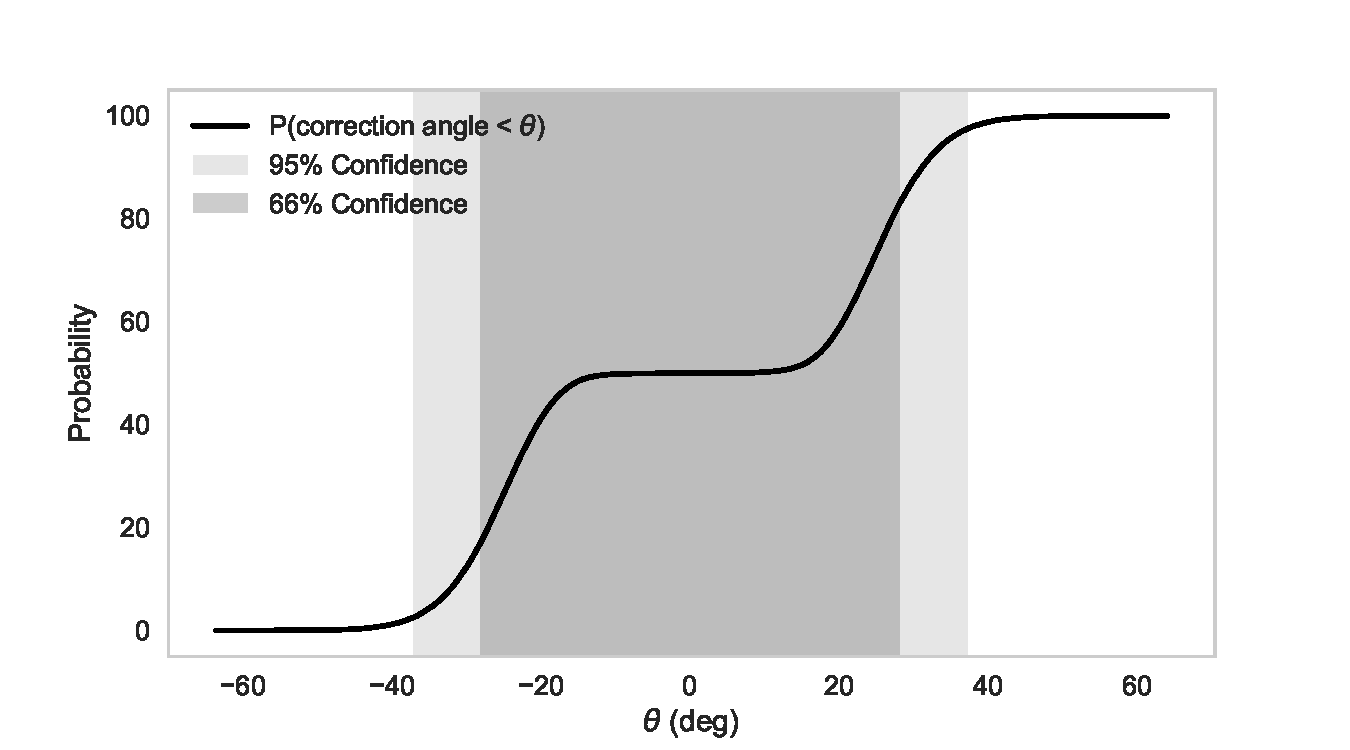
\includegraphics[width=1.0\textwidth]{figures/correction_ecdf.pdf}
\end{figure}


\pagebreak
\begin{algorithm}[H] \label{monte_algo}
\SetAlgoLined
\KwResult{Random samples drawn from distribution of bearing correction angles }
 $m \gets$ input the measured signal amplitude\;
 $\mu_s \gets$ input the cable signal mean\;
 $\sigma_s \gets$ input the cable signal standard deviation\;
 $\mu_b \gets$ input the background mean\;
 $\sigma_b \gets$ input the background standard deviation\;
 $N \gets$ input the desired number of samples\;
 $M \gets$ the maximum iterations for finding a triangle solution\;
 $n \gets 0$\;
 $\bm{\theta} \gets$ An array of length $N$\;
 $n \gets 0$\;
 \While{n < N}{
     $i\gets0$\;
     $keepon \gets$ true\;
     \While{$i < M \And  keepon$}{
          $s \gets$ Draw random value from cable signal distribution\;
          $b \gets$ Draw random value from background signal distribution\;
          \uIf{$\left(m-s\right)^2 \leq b ^ 2 \leq \left(m + s\right)^2$}{
              $u \gets$ Draw randomly from $\left[-1, 1\right]$ with equal probability\; 
              $\bm{\theta}\left[n\right] \gets u \cos^{-1}\left(\frac{m^2 + s^2 - b^2}{2ms}\right)$\;
              $n = n + 1$\;
              $keepon\gets$ false\;
          }
          \Else{
              $keepon\gets$ true\;
          }
          $i \gets i + 1$\;
     }
     \If{$i = M$}{
         $\text{Raise an error indicating that no triangle solutions could be found}$\;
     }

 }
 \caption{Bearing correction Monte-Carlo sampling.}
\end{algorithm}

\pagebreak
\section{Algorithm Implementation}
We chose to implement Algorithm \ref{monte_algo} using the Python language.  Python offers excellent support for data-processing, statistics, and visualization.  We employed the widely-used array-processing and mathematics libraries \texttt{numpy} and \texttt{scipy}, which, due to their array-processing paradigm,  cause the implementation to look quite different from the algorithm pseudo-code.  This section contains our Python implementation of the sampling algorithm.

\subsection{Python Code}

\begin{python}
from scipy.stats import gamma, bernoulli
import numpy as np

def sample_amplitude(mu, sigma, N):
    a = (mu / sigma) ** 2
    scale = sigma ** 2 / mu
    gam = gamma(a, scale=scale)
    return gam.rvs(size=N)

def sample_angle(
        measured, sig_mu, sig_std, back_mu, back_std, N, max_iter=100):
    x_list, n_samples, n_iter = [], N, 0
    while n_samples > 0 and n_iter < max_iter:
        signal = sample_amplitude(sig_mu, sig_std, n_samples)
        background = sample_amplitude(back_mu, back_std, n_samples)
        numerator = measured ** 2 + signal ** 2 - background ** 2
        denominator = 2 * measured * signal
        ratio = numerator / denominator
        ratio = ratio[ratio < 1]
        theta_abs = np.arccos(ratio)
        nn = len(theta_abs)
        signs = 2 * (bernoulli(.5).rvs(nn) - .5)
        theta = theta_abs * signs
        theta = theta[~np.isnan(theta)]
        x_list.extend(theta.tolist())
        n_samples = int(2 * (N - len(x_list)))
        n_iter += 1
    if n_iter >= max_iter:
        raise ValueError('MaxIter encounterd.')
    return 180 * np.array(x_list[:N]) / np.pi

samples = sample_angle(
    measured=2000, sig_mu=1900, sig_std=200, back_mu=900, back_std=200,
    N=100000, max_iter=100
)
\end{python}


\end{appendices}









%%% End document
\end{document}